\documentclass[12pt,pdftex,titlepage]{report}

\author{\textbf{Noah Santschi-Cooney}
\\\\\\\small{Final Year Project - BSc in Computer Science}
\\\\\\\small{Dr. Jason Quinlan}
\\\\\\\small{Department of Computer Science}
\\\small{University College Cork}}
\title{\textbf{Alternative Visualisations of Distributed Tracing data in a complex, large-scale distributed system}}
\date{\vfill\small{3rd April 2020}}

\usepackage[dvipsnames]{xcolor}
\usepackage[utf8]{inputenc}
\usepackage[english]{babel}
\pagenumbering{roman}

\usepackage{graphicx}
\graphicspath{{./assets/}}

\PassOptionsToPackage{hyphens}{url}\usepackage{url}
\usepackage{microtype, caption, copyrightbox, setspace, textcomp, soul, hyperref, listings}
\usepackage{assets/listings-kotlin, assets/listings-graphql, assets/listings-typescript}
\captionsetup[lstlisting]{font={scriptsize},width=0.8\linewidth}
\captionsetup[figure]{font={scriptsize},width=0.8\linewidth}
\setstretch{1.05}

\hypersetup{
    colorlinks,
    citecolor=black,
    filecolor=black,
    linkcolor=black,
    urlcolor=black
}
\lstset{
    frame=leftline,
    basicstyle=\scriptsize\ttfamily,
    keywordstyle=\color{Blue},
    keywordstyle={[2]\color{BrickRed}},
    emphstyle=\bfseries,
    numbers=left,
    numbersep=5pt,
    showstringspaces=false, 
    stringstyle=\color{ForestGreen},
    commentstyle=\color{Gray},
    tabsize=4
}

\makeatletter
\def\@makechapterhead#1{%
  \vspace*{20\p@}% <----------------- Space from top of page to Chapter #
  {\parindent \z@ \raggedright \normalfont
    \ifnum \c@secnumdepth >\m@ne
        \huge\bfseries \thechapter.\ % <-- Chapter # (without "Chapter")
    \fi
    \interlinepenalty\@M
    #1\par\nobreak% <------------------ Chapter title
    \vskip 20\p@% <------------------ Space between chapter title and first paragraph
  }}
\makeatother

\begin{document}
    \maketitle    

    \chapter*{Abstract}
        \begin{spacing}{1.0}
            \addcontentsline{toc}{chapter}{Abstract}
            Modern Internet services are often implemented as complex, large-scale distributed systems. These applications are constructed from collections 
            of software modules that could span many thousands of machines across multiple physical facilities. With the rise of modern Micro-service and 
            Service-Oriented designs, traditional tooling used to monitor application behaviour is no longer viable, especially at scale. 
            
            To understand the flow and life cycle of a unit of work performed in multiple pieces across various components in a distributed system, the concept of 
            Distributed Tracing was born. Distributed Tracing was first introduced to the mainstream world in 2010 after the publication of Google’s Dapper
            paper. Since then, various vendors have come out with their own Dapper-inspired services, most of them based off flame or timeline graphs. 
            
            The goal of this project is dual-faceted:
            \begin{itemize}
                \item Explore and research possible alternative uses and visualisation methods utilising data collected from distributed tracing clients.
                \item Implement one or more of the proposed alternatives.
            \end{itemize}
        \end{spacing}

    \chapter*{Declaration of Originality}
        \begin{spacing}{1.0}
            \addcontentsline{toc}{chapter}{Declaration of Originality}
            In signing this declaration, you are confirming, in writing, that the submitted work
            is entirely your own original work, except where clearly attributed otherwise, and
            that it has not been submitted partly or wholly for any other educational award. I
            hereby declare that:
            \begin{itemize}
                \item this is all my own work, unless clearly indicated otherwise, with full and proper accreditation;  
                \item with respect to my own work: none of it has been submitted at any educational institution contributing in any way to an educational award;
                \item with respect to another’s work: all text, diagrams, code, or ideas, whether verbatim, paraphrased or otherwise modified or adapted, 
                have been duly attributed to the source in a scholarly manner, whether from books, papers, lecture notes or any other student’s work, whether
                published or unpublished, electronically or in print.
            \end{itemize}
            \vspace{10mm}
            Signed: \dotfill
            \\\\
            Date: \dotfill
        \end{spacing}

    \chapter*{Acknowledgements}
        \begin{spacing}{1.0}
            \addcontentsline{toc}{chapter}{Acknowledgements}

        \end{spacing}
        
    \begin{spacing}{1.0}
        \tableofcontents
    \end{spacing}

    \chapter{Introduction}
    \pagenumbering{arabic}
    \setcounter{page}{1}
        \section{Problem}
            Within the last decade, the way modern applications are being built and deployed has changed dramatically. With the shift from collocation to cloud computing,
            virtual machines to containerization technologies, monoliths to micro-services and beyond, software developers have been able to adjust to 
            the monotonical increase in internet traffic, shipping highly scalable, efficient and reliable software that meets the ever-demanding needs of their customers
            with the slew of emerging technologies.

            While this shift has undoubtedly solved many issues with regards to scaling services in terms of both maintainability as feature sets increase and in keeping up
            with an every larger number of online users, it has introduced a whole new suite of problems that needed to be addressed in terms of reliability and application 
            monitoring. With the splitting of monolithic applications into micro-services, the failure points are extended to issues in the network, including but not limited
            to network congestion, DNS resolution errors etc. Developers are ever more inclined to code failure resilience into their applications, falling back gracefully in 
            apprehension of unforeseeable failures.

            As these new distributed system architectures evolved and became ever more widespread, traditional application monitoring tools consistently fell short of providing
            developers and systems operators with the means to gain introspection into systems and their failures in production scenarios\cite{retrospective}. Traditional monolithic systems often
            utilized logging and metrics to gain introspection into the application and for alerting on rules respectively. For such systems, these process-scoped measures often 
            provided good insight into a system, correlating logs on their thread identifier/name as each thread would handle a single request sequentially. As these systems 
            adopted asynchronous execution models, where a request's lifetime may not be confined to a single thread, the previous approach no longer works, making observing
            the behaviour of such systems very difficult unless developers annotated logs with request-scoped identifiers. The final evolution of concurrency in application systems is
            commonly referred to as \textit{distributed concurrency}. This is often associated with micro-services, in which a request is no longer constrained to being executed
            in a single process, but may span multiple processes and even servers. Figure~\ref{fig:concurrency} highlights this evolution, from simple, single threaded applications,
            through to micro-service-like architectures.

            \begin{figure}[htb!]
                \centering
                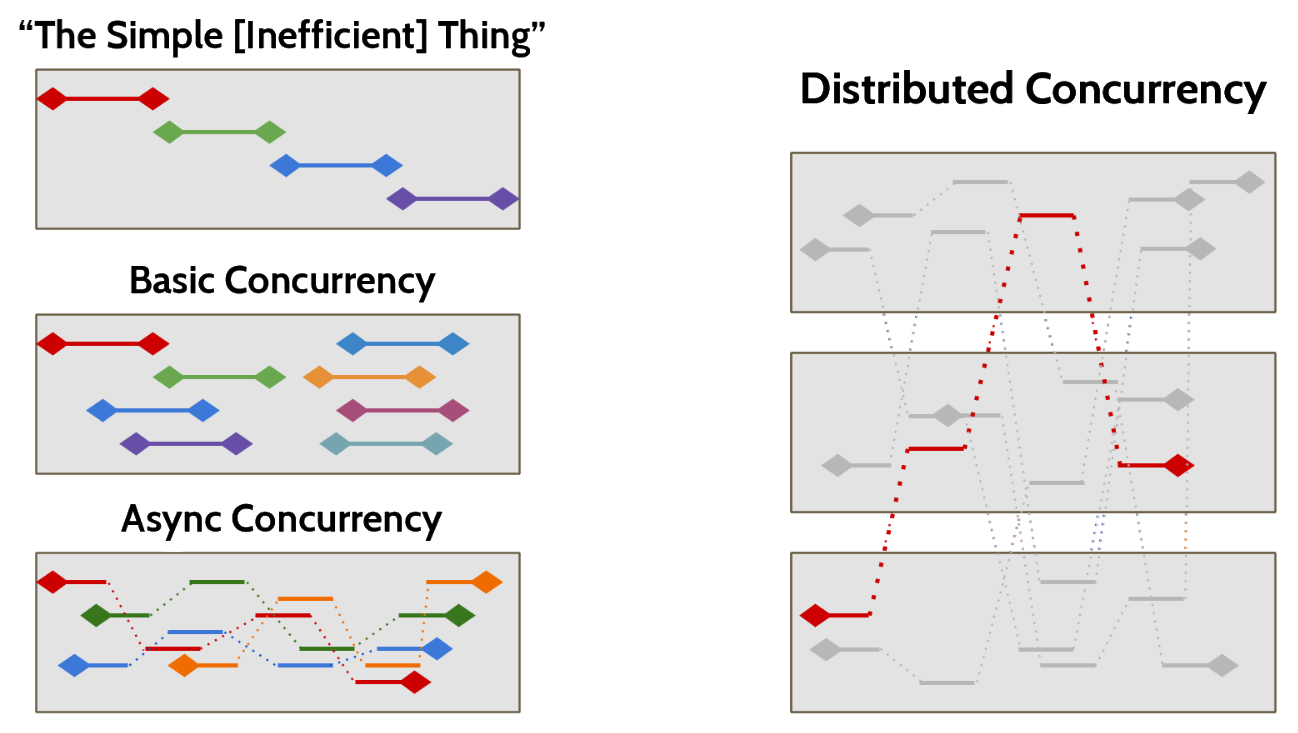
\includegraphics[scale=1.1]{concurrency.png}
                \caption{Evolution of concurrent systems.}
                \label{fig:concurrency}
            \end{figure}
        
        \section{Debuggers}
            In traditional single process applications, debugger tools, both standalone and bundled with integrated development environments (IDEs), are invaluable in their
            use of isolating bugs in codebases of any size. They have the capability to give complete overview of stack and heap allocated variables as well as being able to set
            breakpoints to step through code. Figure~\ref{fig:debugger} highlights the various insights and utilities provided by such tools, including the display of call stacks,
            local and global variables as well as various utilities to step through code at the line and function levels.

            \begin{figure}[hbt!]
                \centering
                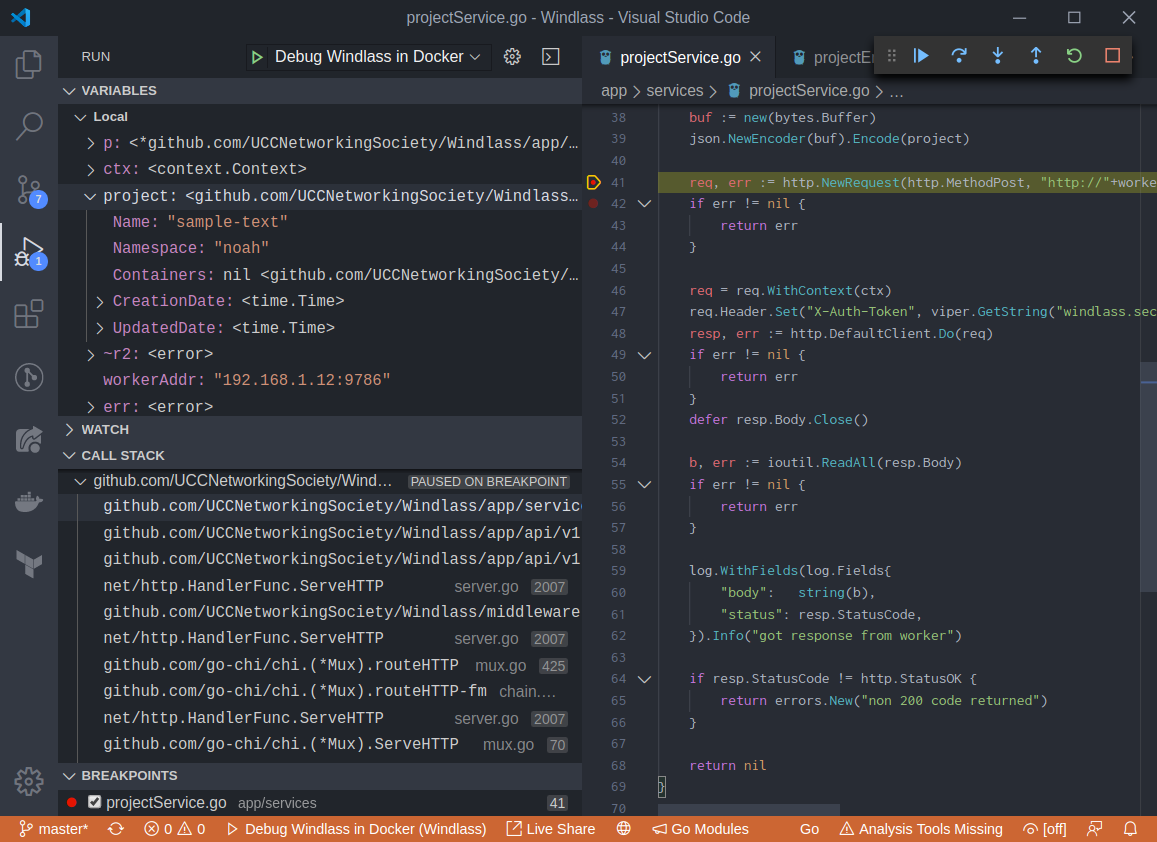
\includegraphics[scale=0.335]{debugger.png}
                \caption{Screenshot of the Visual Studio Code debugger in action. Clockwise, shown are an expandable list of local and global variables, the currently open file view
                with the line currently halted on highlighted along with controls for stepping and finally the function call stack.}
                \label{fig:debugger}
            \end{figure}
            
            However, it is often infeasible to use them in production scenarios due to their nature of halting complete execution of the process.
            This can make them unsuitable for debugging issues that manifest in production that developers are finding difficult to reproduce in development scenarios, as is often
            a common scenario due to subtle parity differences between development and production systems. Section~\ref{sec:debugger} references a project that has made it possible
            for users to use traditional debuggers in a production microservices scenario. The different trade-offs made by the referenced project will be covered,
            as well as the differences between it and the proposed solution outlined in this project.

        \newpage
        \section{Distributed Tracing}
            As traditional tooling is not designed to accommodate for this distributed concurrency system, new methodologies were needed to regain observability into the systems.
            Observing single systems individually, as was done with traditional tooling, no longer painted the full picture of a request as it travels through multiple system 
            components. Distributed tracing systems and platforms build upon the concepts of reconstructing a request from a series of event streams from each component involved
            in the request, with distributed context propagation and aggregation, building causality graphs from a request-centric point of view.

            \begin{figure}[hbt!]
                \centering
                \copyrightbox[r]{
                    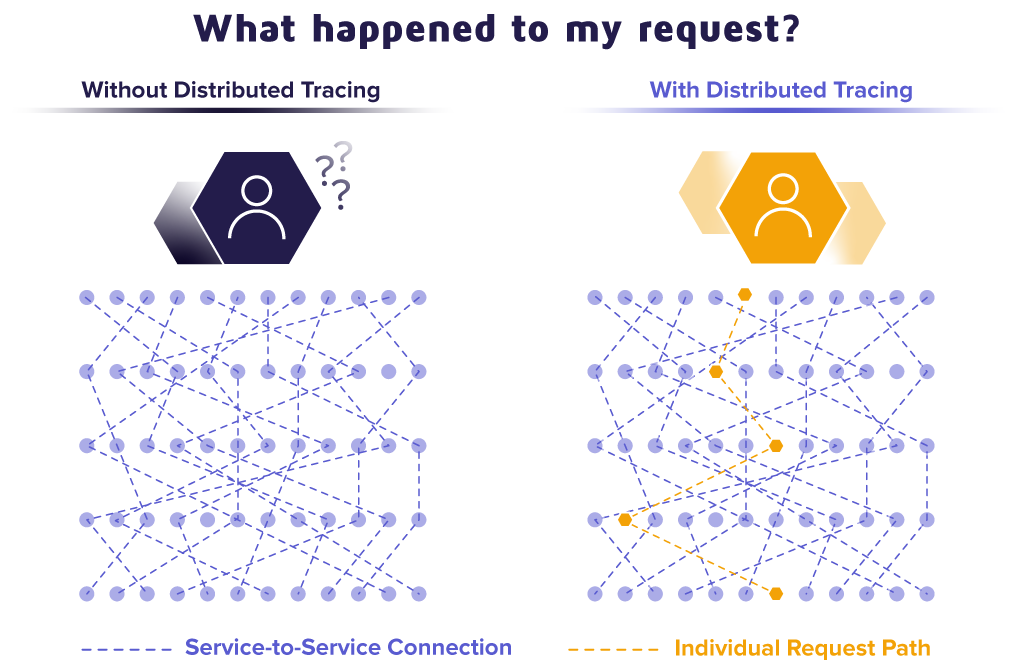
\includegraphics[scale=0.7]{distributed.png}
                }{
                    \tiny{\textcopyright Nitzan Shapira for Epsagon "Introduction to Distributed Tracing". https://epsagon.com/blog/introduction-to-distributed-tracing/}
                }
                \caption{Depiction of a complex distributed system with much inter-connectivity between services.}
                \label{fig:dist}
            \end{figure}

            Code is instrumented at various points of interest, recording annotated events with metadata such as the user ID associated with the request, SQL statements being 
            executed on a database etc. These events are often shipped to a collector/exporter, from which they are either stored in a database or sent to a hosted vendor, such as
            LightStep or Honeycomb, after which they can be queried, retrieved and displayed.

        \section{Motivation \& Goals}
            As distributed tracing is still a relatively new idea and only as of recently gathering mainstream interest in the industry, research and advancements on the topic are 
            as of yet still sparse. Current vendors often provide a limited set of capabilities and operations that can be performed on the data output from instrumented distributed systems,
            most commonly simple expandable \textit{gantt charts} or, less commonly, simple, mostly static, service dependency graphs that operate on pre-aggregated data that offer little 
            value and utility in debugging at a detailed level, resulting in systems that can only be grouped as monitoring solutions rather than observability solutions.
            
            To further research in this field, this project will attempt to explore alternative and, ideally, improved ways of consuming and presenting the data from instrumented
            applications. Two ideas were planned to be explored and, if possible, implemented as proof of concepts:

            \begin{itemize}
                \item Advancements in Service Topology graphs
                \item Editor Debugger integration                
            \end{itemize}

            % TODO:
            The viability and findings of both explored options will be discussed, with performance benchmarks where relevant being presented to highlight the feasibility of different
            approaches under potential real-world constraints and limitations.

        \section{Project Summary}
            This project builds upon the concepts of distributed tracing, exploring ways to provide novel and high-value derivable ways of visualising and presenting distributed tracing
            data to developers. Modern standards, tools and integrations will be utilized to test the viability of less common and unexplored visualisations of distributed tracing data
            as well as expanding on current approaches.

            In Chapter 2, the history of distributed tracing will be introduced, while also covering some common vocabulary relevant to the topic and where they originated. It will also
            cover some of the standards that this project builds around. In Chapter 3, the project architecture design choices will be discussed and how they impacted the project, ranging
            from the frontend frameworks chosen to the backend API and supporting services that power the various implementations, as well as covering the implementation details of the various
            components that resulted from the work done. Finally, the different visualisations will be evaluated on the value the provide as well as the feasibility of utilizing them in real-world
            scenarios. Chapters 5 and 6 will draw the writeup to a conclusion, detailing the closing thoughts and putting forward ideas for future work on the ideas explored in this project.

    \chapter{Background}
        \small{In this chapter we will briefly cover the history of distributed tracing, the major tools and specifications that lay the foundation of what distributed tracing is today,
        as well as upcoming standards that aim to modernise and solve the short-comings of what came before. This will be followed by a summary of some commonly adopted visualisations
        of distributed tracing data as well as the work that will be carried out in furthering research into visualising tracing data.}

        \section{History \& Future}
            \subsection{Dapper}
                Released in April 2010, Google published a paper describing the design decisions behind an in-house implementation 
                of distributed tracing, named Dapper. It is commonly believed that this paper describes the common ancestor to 
                many tools that implement a form of distributed tracing.

                The Dapper paper introduces some of the core primitives that underpin modern day standards. Most notable are the concepts
                of a directed acyclic graph (DAG) called a \textit{trace tree} and its nodes, which are referred to as \textit{spans}. 
                The trace tree forms a relationship between spans, not unakin to a tree of stack frames that may be generated by
                gathering stack frames over time, albeit generally at a much higher level than at the level of individual subroutine calls. 

                Figure~\ref{fig:dappertrace} illustrates a trace tree with five spans. Each span is shown to contain 3 specific pieces of
                metadata alongside the start and end timestamps necessarily to reconstruct the temporal relationships: a human-readable
                \textit{span name}, an integer \textit{span ID} and an integer \textit{parent ID}. The latter two
                data points are used to reconstruct the relationship between individual spans. A span without a parent ID becomes the 
                \textit{root span} of a trace tree. Not shown is another important but, as of right now, not relevant piece of metadata, the 
                \textit{trace ID}, which is common amongst all spans within a single trace tree.

                \begin{figure}[htb!]
                    \centering
                    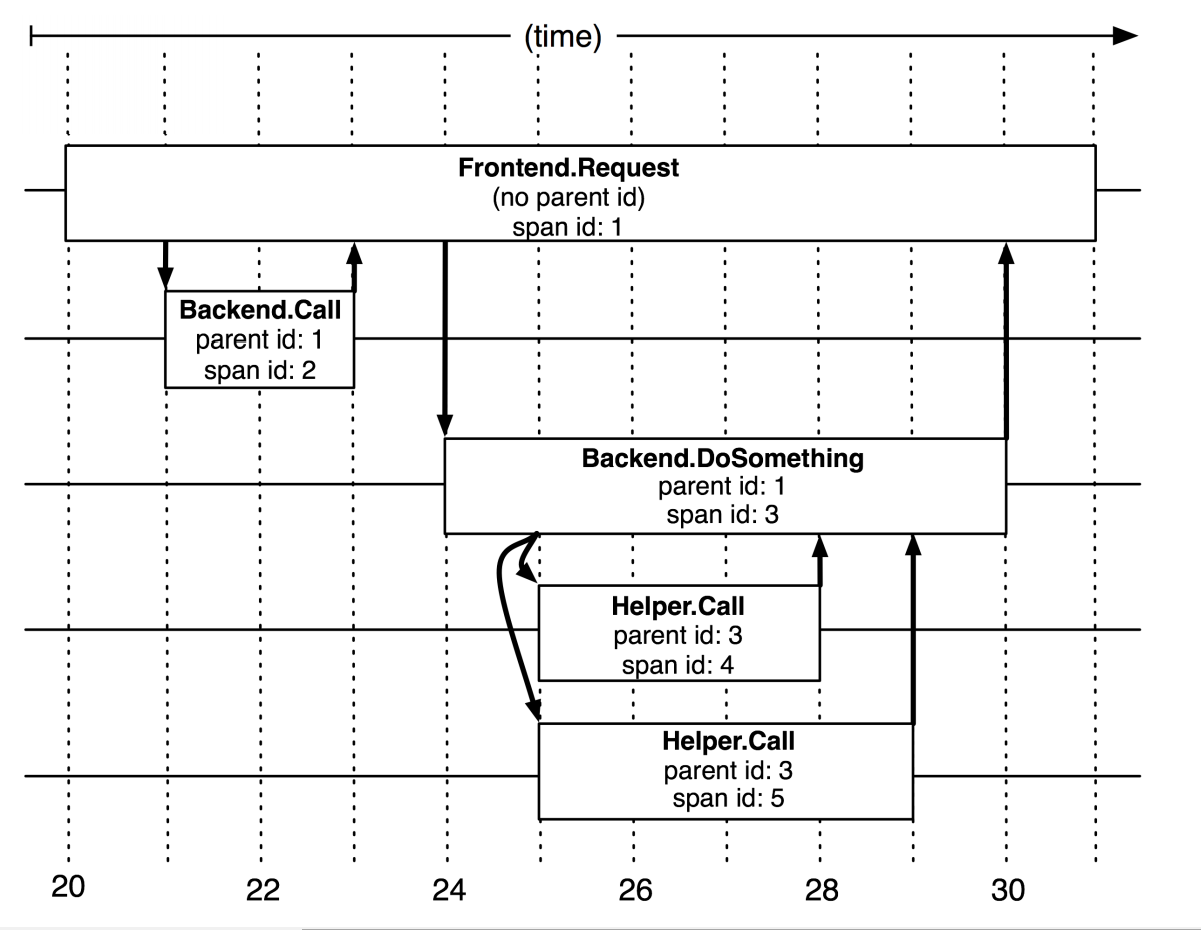
\includegraphics[scale=1.2]{dappertrace.png}
                    \caption{The relationships between traces in a trace tree. Each span contains its span identifier as well as that of its parent. 
                    The root span contains no parent span identifier, signifying that it is the root span.}
                    \label{fig:dappertrace}
                \end{figure}

                As described thus far, Dapper trace trees allow for a detailed view of the relationships of distributed systems within
                Google. When using this data for debugging or performance analysis, it can often be convenient or even necessary to 
                have additional context surrounding a trace tree or its individual spans. As such, the paper describes a simple API 
                through which application developers can provide a combination of two types of annotations: timestamped textual annotations
                and key-value, allowing for defining arbitrary equivalence classes between traces which can be operated upon in the analysis
                tools.

            \subsection{OpenTracing}
                The OpenTracing\cite{opentracing} project's inception came about in October 2015, it has since become a project under the 
                Cloud Native Computing Foundation in 2016, created to standardize a set of vendor neutral and programming language agnostic
                application programming interfaces (APIs) for instrumenting code for distributed tracing. Heavily inspired by the Dapper
                paper, it borrows many of the nouns and verbs outlined in the Dapper paper, including \textit{traces} and \textit{spans}.
                Dapper's timestamped annotations are referred to as \textit{logs} in the OpenTracing specification, while the key-value pairs
                are named \textit{tags}. 

                The OpenTracing API also specifies how a trace cross process boundaries, so that spans created in different processes can be
                associated with a common trace tree. This was named the \textit{span context} and at its most basic level contains the 
                overlying trace ID as well as the current span ID. With this, new spans generated across process boundaries have the ability to
                to specify their parent span as well as their common trace, without propagating an entire span, which may prove costly as more
                tags and logs are attached to a span.

                Figure~\ref{fig:opentracing} shows a timeline based visualisation of where the different components of the OpenTracing API interface are utilized in
                the larger picture of creating a span through use of distributed context propagation in the span context construct to build the span tree across
                process and network boundaries.
                
                \begin{figure}[hbt!]
                    \centering
                    \copyrightbox[r]{
                        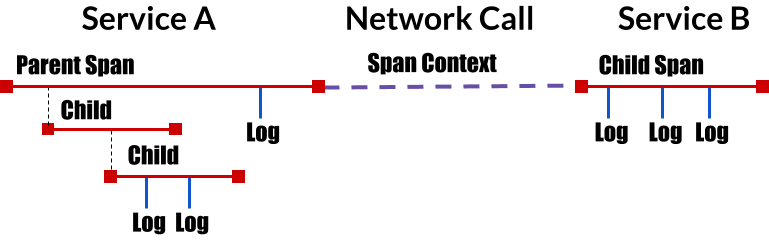
\includegraphics[scale=0.45]{opentracing.png}
                    }{\tiny{\textcopyright OpenTracing "OpenTracing Overview"}}
                    \caption{Infographic visualising the different components that make up the OpenTracing API interface and how they relate to different services
                    and the network}
                    \label{fig:opentracing}
                \end{figure}

                As there are multiple output sinks which can consume OpenTracing data, from self hosting services such as Jaeger to hosted vendors like LightStep, and given that
                different platforms may have different, vendor-specific options for operations such as access control, authorization etc, vendors provide different mechanisms
                and attributes for creating instances of OpenTracing API \textit{tracers} implementations. Listings~{\ref{lst:ddogtrace}} and {\ref{lst:jaegertrace}} highlight how defining a tracer
                for Datadog and Jaeger differ due to different requirements and additional options available to each. On top of this, each tracer implementation defined different HTTP header 
                keys and encodings used to propagate span context across network and process boundaries. This was a source of problems, especially in distributed systems
                that included services over which a company may not have control over the source code, where different codebases may use different tracer implementations, causing context
                propagation to fall apart. This is one of the issues that the \textit{OpenTelemetry} project, outlined in Section~{\ref{sec:opentele}}, attempts to resolve.

                \begin{spacing}{1.0}
                    \begin{lstlisting}[caption=Example Go language snippet of instatiating a Datadog OpenTracing compatible tracer., language=Go, gobble=24, label={lst:ddogtrace}]
                        package main

                        import (
                            "gopkg.in/DataDog/dd-trace-go.v1/ddtrace"
                            "gopkg.in/DataDog/dd-trace-go.v1/ddtrace/opentracer"
                            "github.com/opentracing/opentracing-go"
                        )

                        // Start a Datadog tracer, optionally providing a set of options,
                        // returning an opentracing.Tracer which wraps it.
                        t := opentracer.New(
                            tracer.WithAgentAddr("host:port"),
                            tracer.WithServiceName("sample-text"))

                            // Use it with the OpenTracing API, setting it as global.
                        opentracing.SetGlobalTracer(t)
                    \end{lstlisting}
                \end{spacing}

                \begin{spacing}{1.0}
                    \begin{lstlisting}[caption=Example Go language snippet of instatiating a Jaeger OpenTracing compatible tracer., language=Go, gobble=24, label={lst:jaegertrace}]
                        package main

                        import (
                            "github.com/uber/jaeger-client-go"
                            "github.com/uber/jaeger-client-go/transport"
                            "github.com/opentracing/opentracing-go"
                        )

                        // Start a Jaeger tracer, supplying the sampling strategy and the
                        // reporter configuration.
                        t, closer := jaeger.NewTracer(
                            "sample-text",
                            jaeger.NewConstSampler(true),
                            jaeger.NewRemoteReporter(transport.NewHTTPTransport("host:port")))
                        defer closer.Close()

                        // Use it with the OpenTracing API, setting it as global.
                        opentracing.SetGlobalTracer(t)
                    \end{lstlisting}
                \end{spacing}

            \subsection{OpenTelemetry}
            \label{sec:opentele}
                The OpenTelemetry\cite{opentelemetry} project came about as a result of the merging of two previous projects, namely the previously mentioned OpenTracing
                project as well as OpenCensus project. The OpenCensus project originated from Google and had many similar goals to OpenTracing. Alongside having an interface
                for distributed tracing gathering, it also supported instrumenting applications to output application metrics data. To reduce the fragmentation in having
                two independent APIs for distributed tracing, the two projects decided to merge into one standard going forward. At the time of writing, support for OpenTelemetry
                is still very sparse, due to the fact that it is still a very new specification set, while still being largely backwards compatible with both OpenTracing and 
                OpenCensus, providing API bridges to maintain compatibility. 

                The OpenTelemetry API improves upon OpenTracing by introducing a set specification for context propagating, defining the header keys used to identify specific values 
                relevant to propagating span context through process boundaries, created as a W3C specification. In OpenTracing API implementations, different vendors would use different 
                keys to denote values such as the trace ID etc in, for example, HTTP headers. This would break the context chain if different codebases used different vendor implementations
                in a service dependency graph. By demoting vendor libraries to providing simple \textit{exporters} that define how distributed tracing data is exported to backend systems
                rather than having them provide tracer implementations like the way it was done with the OpenTracing API, and introducing a vendor-agnostic \textit{collector} implementation that 
                will become the single service that defines how distributed tracing data and metrics are received, processed and exported, the OpenTelemetry project achieves a better level of 
                interoperability between codebases, removing the need to operate and maintain multiple agents for various distributed tracing data formats, exporters and metrics backends.

                \begin{figure}[hbt!]
                    \centering
                    \copyrightbox[r]{
                        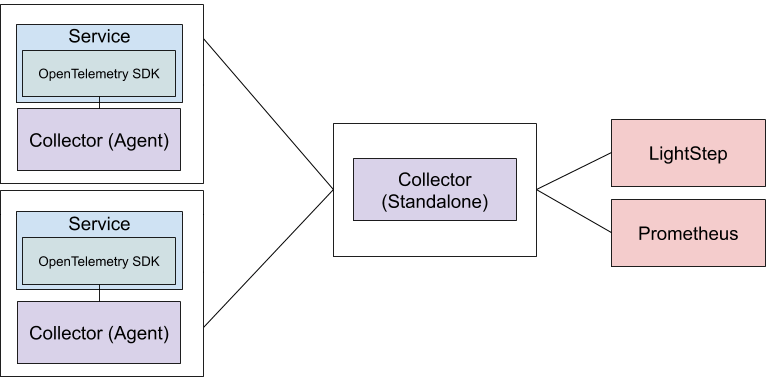
\includegraphics[scale=0.48]{opentelemetry-exporter.png}
                    }{\tiny{\textcopyright{LightStep "OpenTelemetry 101: What is an Exporter?"}}}
                    \caption{A high level overview of a typical OpenTelemetry setup, with services hooking into the OpenTelemetry SDK to output telemetry to
                    OpenTelemetry Collectors, which themselves forward data to the standalone Collector sink, which is configured to send metrics to a \textit{Prometheus}
                    server and distributed tracing data to the LightStep API.}
                    \label{fig:otexporter}
                \end{figure}

        \section{Visualisations of Distributed Traces}
            All this telemetry data would be of little use if it wasn't consumed in some manner. As distributed tracing has only become a more
            prominent topic in the industry in the last half decade, the set of visualisations that exist and are commonly employed is still rather
            small in number. In this section, we will discuss some of the most common forms of visualisations, leading up to the methods explored 
            in this project and how they differ or build upon previous efforts.
        
            \subsection{Flame Graph/Gantt Chart}
                By far the most commonly adopted visualisation is a style of graph closely modeled after the \textit{flame graph}\cite{lightsteptrace}
                \cite{datadogtrace} style, closely resembling Figure~\ref{fig:dappertrace}. It also goes under various other names, 
                examples ranging from \textit{gantt chart}\cite{yuritrace} to \textit{waterfall view}\cite{honeycombtrace}. An example of 
                such can be seen in Figure~\ref{fig:jaeger}, which shows a screenshot of the Jaeger distributed tracing platform user interface. 
                
                Each entry in the graph corresponds to a span in the overall trace tree. They can be expanded to display the logs and tags associated with a 
                given span. The value that can be derived from this visualisation has resulted in large adoption of the flame graph style in distributed 
                tracing providers and platforms, leading many to consider it the de-facto visualisation option for tracing data.

                This form has existed since Dapper, with the visualisation being present in the Dapper user interface. While being the most widespread visualisation
                form for distributed tracing, being able to provide a low-level view into the form of an individual trace, it has started to gather criticism for being
                too low-level, especially earlier in the debugging process. This is largely said to be down to two reasons: 1) to make a trace useful, a user of a distributed
                tracing service must first know what they are looking, knowing what trace they need to look at and 2) if starting from a single trace, a user needs to be able to work
                upwards and deal with the data set in aggregate, finding metadata that is common across all events that correlate with certain problematic system behaviour. This has
                sparked a shift in how trace data is used, with services such as Honeycomb.io providing forms of trace aggregation to assist in users being able to find what is 
                correlated for a given issue across multiple traces\cite{traceaggregate}.
        
                \begin{figure}[htb!]
                    \centering
                    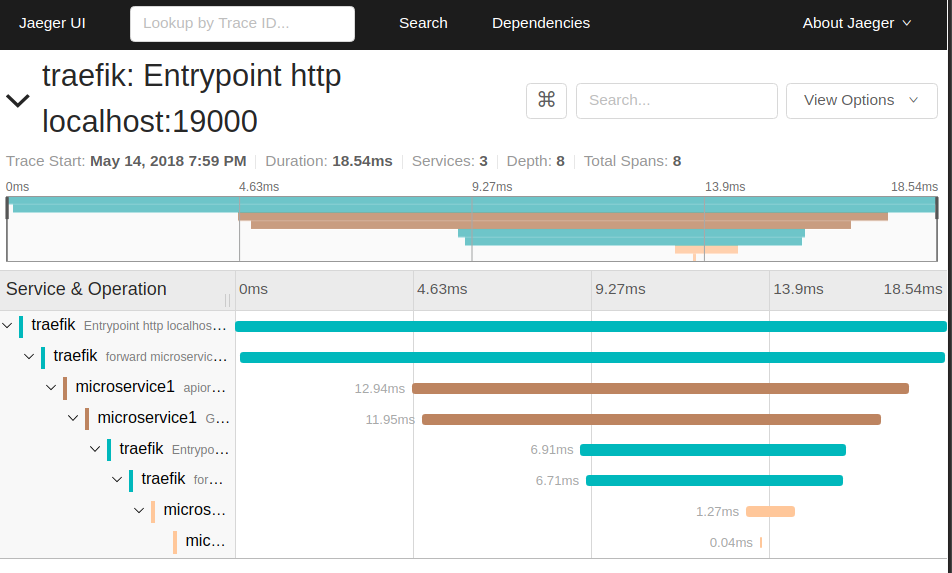
\includegraphics[scale=0.4]{jaeger}
                    \caption{Example of the visualisation of tracing data in Uber's Distributed Tracing platform, Jaeger\cite{jaeger}, providing
                    a flame graph/gantt chart visualisation of a single trace. Each horizontal bar represents a single span while each colour denotes
                    a different service, with three services being displayed.}
                    \label{fig:jaeger}
                \end{figure}
    
            \newpage
            \subsection{Service Topology}
                This was the first alternative explored as part of the final year project. It has become more widespread in its adoption amongst 
                different vendors with varying levels of sophistication\cite{risingstacktopo}\cite{kialitopo}. Most commonly, a force-directed 
                graph is employed for its aesthetically pleasing properties however dominance drawing styles are also prominently used.
        
                A basic service topology graph can give a quick overview of the dependencies between different services in a distributed
                system. For developers and administrators to derive tangible value from such a visualisation outside of a pretty picture, the graph
                needs to provide useful consumable data that can aid in the debugging and monitoring of the behaviour of distributed systems in production
                scenarios. Coupled with an overview of metrics for each node and edge in the graph, such as error rates or response times,
                they have proven to be a valuable monitoring tool.

                \begin{figure}[hbt!]
                    \centering
                    \copyrightbox[r]{
                        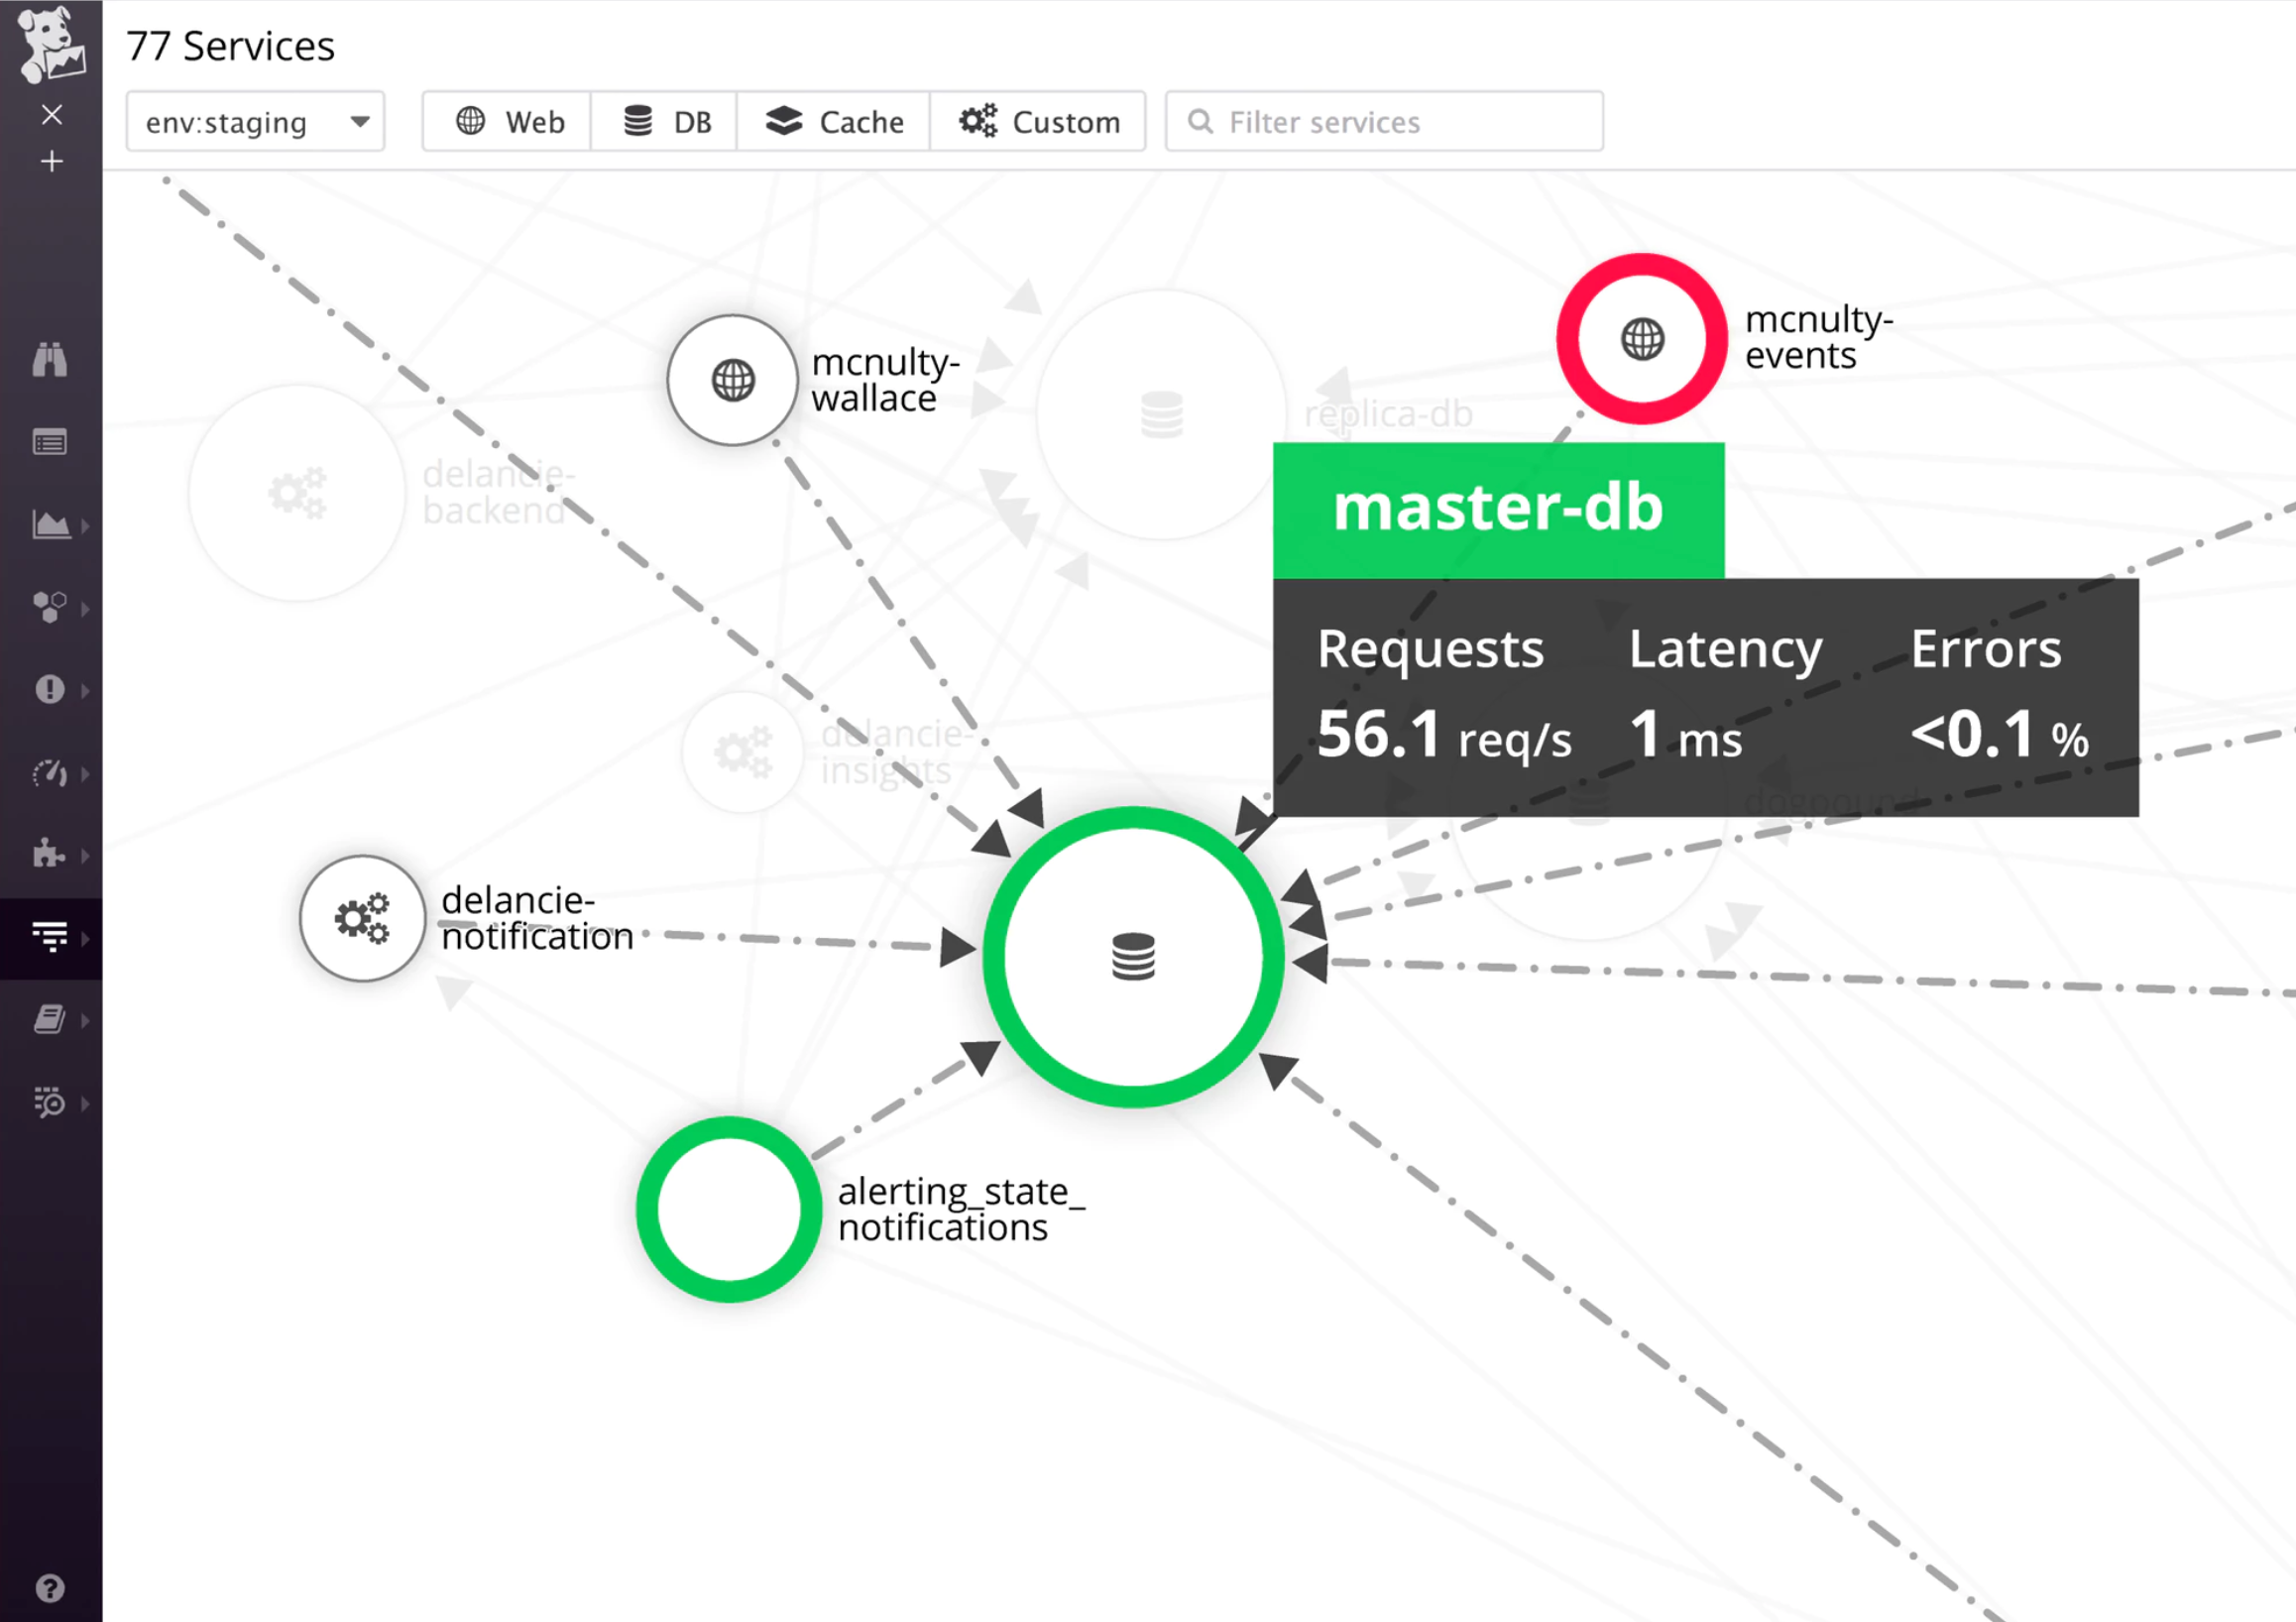
\includegraphics[scale=0.3]{datadog-clustered-map.png}
                    }{\tiny{\textcopyright{Datadog - Introducing the Service Map in Datadog. https://www.datadoghq.com/blog/service-map/}}}
                    \caption{Metrics-based service topology visualisation, showing the dependencies between different services in a distributed system as well as
                    aggregated metrics relating to each node, such as request rate, latency and error percentage.}
                \end{figure}
                
                To bring such visualisations beyond monitoring and into the realm of observability, there is a need for a more dynamic and granular 
                system, not operating on pre-aggregated metrics. The ability to generate views based on arbitrary attributes would allow for users 
                of the system to create more germane and focused graphs based on their needs, such as grouping by high cardinality fields like end-user IP address, 
                error rates, response times and any other field associated with the events consumable by the system\cite{doingitwrongtopo}. The viability and 
                value of creating such a system will be explored, discussing the features that would be expected of such a visualisation, what operations on the
                data it would support to present users with dynamic and powerful data representations with the addition of being able to replay individual traces 
                instead of being presented an aggregated view. The visualisation ideas explored in the \textbf{Design \& Implementation} chapter took inspiration from
                the Massachusetts Bay Transit Authority (MBTA) data visualisation project\cite{mbta} and Cindy Sridharan's section on service topology maps in her blog 
                post titled \textit{Distributed Tracing - we've been doing it wrong}\cite{doingitwrongtopo}, which lay the foundations for the discussions on 
                expanding the ideas outlined in the blog post with respect to the current implementations of monitoring-oriented service topology maps.
    
            \subsection{In-Editor Debugger Integration}
            \label{sec:debugger}
                This is the second and final alternative explored as part of the project. The goal of this visualisation alternative was to
                experiment with the attaching of runtime information to the tags of spans and processing said data in such a way that in-editor
                debugging tools can consume it to step through code akin to attaching to a local process using the same debugging tools.
        
                Unlike traditional debuggers such as the \textit{GNU Project Debugger} (gdb)\cite{gdb}, where stepping through code requires complete
                halting of program execution, using the runtime data attached to trace data allows for after-the-fact, non-blocking stepping
                through code, at an expectedly lower resolution than what can be achieved through traditional, halting debuggers.
        
                A similar concept exists that works in a fundamentally different way and makes different trade-offs to achieve a similar goal.
                Named \textit{Squash}, by \textit{Solo.io}, it more closely follows the style of traditional debuggers by providing a way of attaching
                to processes in a microservices system in a blocking manner, allowing for stepping through code at the same level of granularity as 
                traditional debuggers, along with the same features such as viewing and modifying local and global variables, setting breakpoints etc.
                As such, it retains many of the same downsides, such as the inherent full-application halting when breakpoints are hit and when stepping
                through code. Due to the nature of how it works, it is also a less generic solution, requiring custom support for platforms in which applications
                may be deployed as well as custom support for individual debugger runtimes, such as gdb, delve\cite{delve} etc. At the time of writing, it supports Kubernetes, 
                OpenShift and Istio in the application orchestration and service mesh group of services, and delve, \textit{Java Debug Wire Protocol}\cite{jdwp}, 
                NodeJS\cite{nodejs} and \textit{Python Tools for Visual Studio debug server}\cite{ptvsd} in the debugger runtimes group of tools.

                This is in contrast to the concept explored in this project. It trades the granularity of being able to step through code on a line-by-line basis and
                the more powerful variable inspection capabilities for a fully non-blocking and application-deployment agnostic method of being able to step through code
                of the lifetime of a request at any stage after the fact. It does not rely on existing debugger runtimes or tools outside of the requirements for collecting,
                storing and retrieving distributed tracing data and being able to query the application runtime or employing other heuristics for gathering runtime data
                on the call stack information.
        
        \section{Conclusion}
            Even though distributed tracing has been around for just short of over a decade, it has only seen significant adoption with the inception of OpenTracing, unifying a set
            of standards to improve the experience of adopting distributed tracing. The upcoming OpenTelemetry standard aims to take what made OpenTracing as successful as it is and improve
            the developer experience further by making the distributed tracing API more vendor neutral and flexible. While the standards are evolving, services and platforms that consume
            and visualise distributed tracing data have been mostly basing themselves on a small set of visualisation that have remained largely unchanged over the years, often pre-aggregating
            data on ingest, after which vital context surrounding the data is lost, or providing only minimal operations that can be performed on the data, resulting in services that fail
            to provide deeper insight beyond service monitoring by providing data without enough context or not providing the tools to dynamically work up from individual traces and effectively
            find correlations in the data.
                    

    \chapter{Design \& Implementation}
        \small{In this section, the different technical aspects will be covered, design decisions and components that played a role throughout the projects lifecycle.
        This will include third party services and platforms, and the roles they played. Implementation details such as languages and libraries used are discussed in the
        \textbf{Implementation} sections. The \textbf{Designs and Architecture} sections cover protocols, APIs and interfaces that underpin the project, as well as the 
        design and architecture decisions of the explored ideas in a language agnostic manner.}

        \section{Designs and Architectures}
            \subsection{Distributed Tracing API}
                The OpenTracing API standard was chosen as the foundation for this project. This decision was made due to the large language support and comprehensive open
                source tooling built around the OpenTracing API in contrast to OpenCensus or, particularly, OpenTelemetry, as well as the students prior experience with OpenTracing.

                OpenTelemetry was initially considered as an alternative choice instead of OpenTracing, but was ultimately decided against due to it still being a very new
                standard, with OpenTracing having much more comprehensive support and documentation resources from both application libraries and distributed tracing tools.
                OpenTelemetry was still in pre-beta stage when this final year project was started, with the beta releases for a number of instrumentation libraries having been
                announced in March 30th 2020. This would have added huge delay in being able to commence the project on top of additional complexity being introduced than what exists 
                in a simple development-oriented OpenTracing setup with the OpenTelemetry backing components, including the collector and exporters.

                Potential explorations around the OpenTelemetry API are discussed in the \textbf{Future Work} section.

            \newpage
            \subsection{Supporting Services}
                As both explored ideas will be interacting with distributed tracing data, there are two pieces to the puzzle of having a set of traces to work with.
                Firstly, a way of collecting trace data from applications is needed, and secondly, the database into which the data is persisted.
                
                The distributed tracing platform, Jaeger, was chosen for this project. Jaeger is wholly self-hostable, providing a convenient setup for single-machine development purposes with
                a single, all-inclusive binary available from the distribution archives, as well as a pre-built \textit{Docker} image published to DockerHub. The full Jaeger package,
                available in whole in the aforementioned all-inclusive formats, includes the trace collector, trace search and visualisation user interface and agent.

                By default, the all-in-one Jaeger distribution stores all trace data in-memory. For convenience to persist data in between machine reboots, the JSON document search engine
                database, \textit{Elasticsearch}, was chosen as the storage backend for Jaeger, as one of two possible choices alongside \textit{Apache Cassandra}, a column store document
                database. The Backend API, discussed later in this chapter, interfaces with the Elasticsearch database as the source of truth for the trace data. A complementary user interface
                for Elasticsearch, maintained by the developers of Elasticsearch, \textit{Kibana}, was used throughout the development of the project to view the raw trace data as it is 
                represented in the database.

            \subsection{Backend API}
                To query for and transform the distributed tracing data stored in Elasticsearch, an HTTP API was developed for the two codebases of the ideas explored to interface with.
                It implements a GraphQL HTTP API server, the concepts of which are explained in detail below, to fetch the trace data from Elasticsearch. Figure~\ref{fig:arch} illustrates
                the final design of the architecture, showing where the backend API, trace data consuming clients (the implementations of the ideas that will be discussed), trace data collectors
                outlined in the previous section as well as the applications that emit trace data fit into the picture.

                \subsubsection{GraphQL}
                    As an alternative to traditional RESTful HTTP services, GraphQL is both a query language and a server-side runtime for executing queries against a defined data schema
                    laid out by the type system. The type system can be shared between both servers and clients alike, allowing for a common, known data schema. The data schema consists of 
                    user defined object types representing the data, as well as two special types: the \textit{Query} type and the \textit{Mutation} type. These define the entrypoints into
                    the GraphQL server, allowing for the fetching and modification of data by a named entrypoint. These entrypoints can take a defined set of arguments and return any type
                    detailed in the schema, of which any argument and the return type may be denoted as being optional.

                    \begin{lstlisting}[caption={The base GraphQL schema, defining a query and data types for the trace data.}, language=GraphQL, gobble=24]
                        type Query {
                            findTrace(traceID: String!): Trace
                        }

                        type Trace {
                            traceID: String!
                            spans: [Span!]!
                        }

                        type Span {
                            traceID: String!
                            spanID: String!
                            parentSpanID: String
                            duration: Int!
                            startTime: Int!
                            operationName: String!
                            serviceName: String!
                            logs: [LogPoint!]
                            tags: [Tag!]
                        }

                        type LogPoint {
                            timestamp: Int!
                            fields: [LogPointField!]!
                        }

                        type LogPointField {
                            key: String!
                            type: String!
                            value: String!
                        }

                        type Tag {
                            key: String!
                            type: String!
                            value: String!
                        }
                    \end{lstlisting}
                    \bigskip
                    
                    One of GraphQLs improvements over traditional REST is the ability to specify fields to \textit{resolve} in the server-side runtime engine. Besides preventing
                    under- and over-fetching, this also allows for the ability to selectively augment the returned data, adding extra fields or even changing existing ones on-demand,
                    all within the same query while not incurring the costs for clients that do not request them. Listing~\ref{lst:graphTrace} shows an example of selective field
                    resolving. The second query also requests the \texttt{spans} field, which could have a range of effects on the server e.g. performing an extra SQL \texttt{JOIN}
                    statement, while also resulting in potentially more data being sent down the wire.

                    \begin{lstlisting}[caption={GraphQL query to fetch a trace object and the span ID of each of its spans vs a query to fetch the trace object, its spans and every
                        tag of every span.}, label={lst:graphTrace}, language=GraphQL, gobble=24]
                        {
                            query findTrace(traceID: "asdf") {
                                traceID
                                spans {
                                    spanID
                                }
                            }
                        }

                        {
                            query findTrace(traceID: "asdf") {
                                traceID
                                spans {
                                    spanID
                                    tags {
                                        key
                                        value
                                    }
                                }
                            }
                        }
                    \end{lstlisting}

                \subsubsection{Interfacing with the Database}
                    As the decision was made to use the Jaeger tracing platform backed by Elasticsearch for this project, the backend server must interface with Elasticsearch
                    to be able to serve the data to the API clients that make up this project. Under these circumstances, this project could be potentially used in production
                    by teams that host a Jaeger tracing platform on their infrastructure with Elasticsearch. The backend must simply support connecting to the database, building 
                    JSON queries at either an abstracted or low level and finally being able to execute those queries against the database. Elasticsearch has first-party libraries
                    for a  large number of languages, and given Kotlin's interoperability with Java, the backend makes use of the Java Elasticsearch client library. Adding support 
                    for Apache Cassandra database would be trivial, however outside of the scope of this project.

                    While the Jaeger tracing platform is commonly employed by development teams, vendor hosted distributed tracing systems also have seen large adoption due to the 
                    fact that it allows teams to not worry about maintaining an instance of Jaeger in their infrastructure, either due to convenience, monetary costs needed to host
                    the Jaeger platform or having to maintain extra services. These vendors often do not provide a public API for querying and fetching trace data. Discussion around
                    possible solutions for these scenarios can be found in the future works section. The rest of this report works under the assumption of the Jaeger tracing platform
                    being employed, either as the sole distributed tracing system or complementary to a vendor hosted solution. 

                \bigskip
                \begin{figure}[hbt!]
                    \centering
                    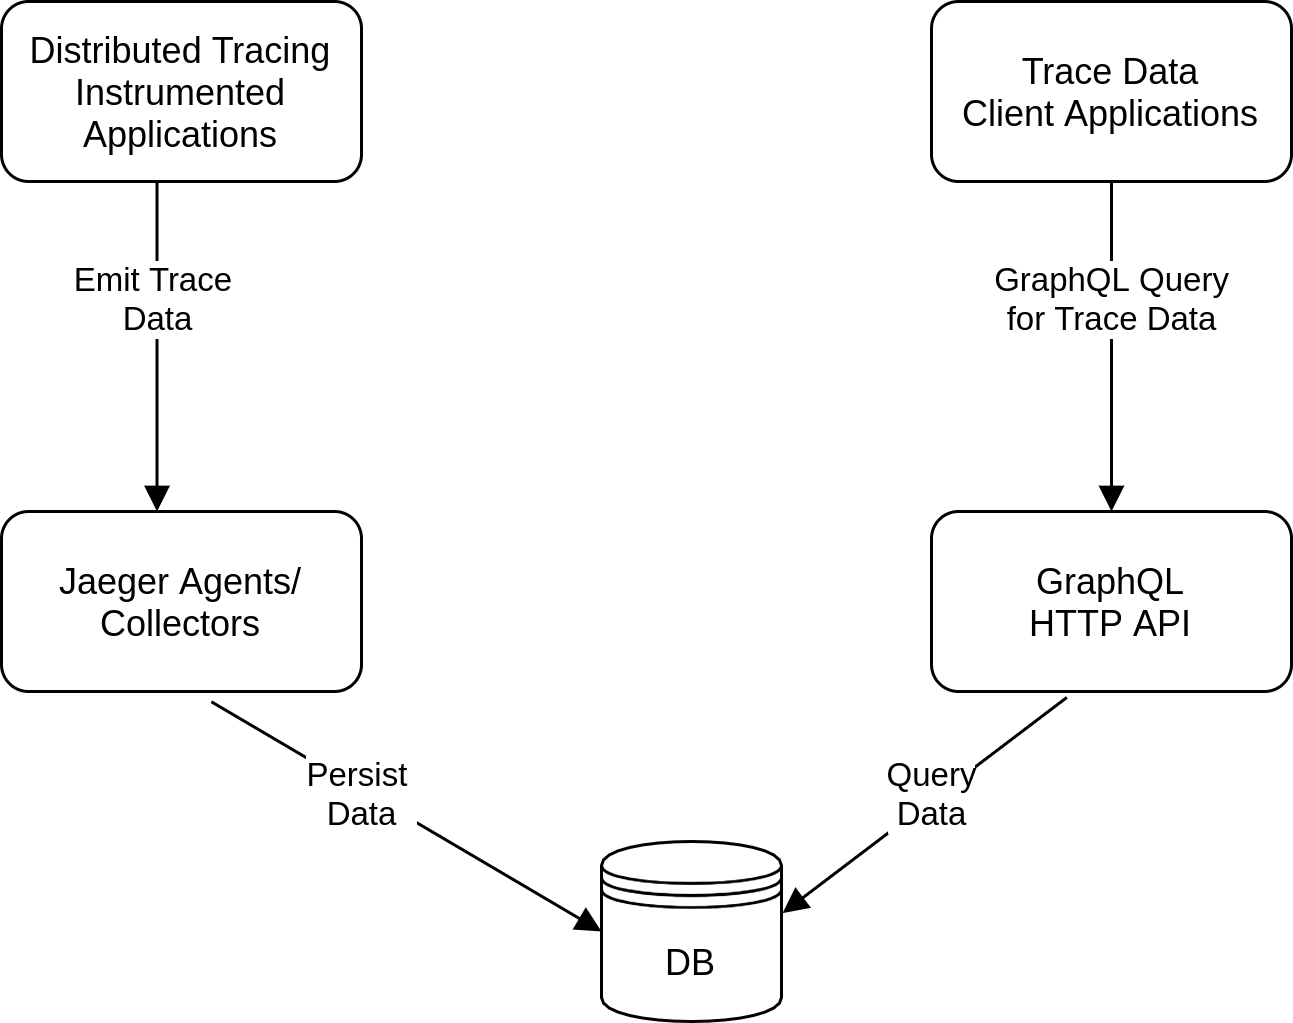
\includegraphics[scale=0.2]{arch.png}
                    \caption{Basic diagram illustrating the architecture design for a sample system, including applications instrumented to emit trace data, the Jaeger agents and/or collectors,
                    the database in which trace data is persisted and the GraphQL HTTP API that the clients such as those implemented as part of this project interact with to obtain trace data.}
                    \label{fig:arch}
                \end{figure}

            \subsection{Debug Adapter}
                For this part of the project, it was decided to develop the idea of integrating the telemetry from instrumented applications into the debugger API of Visual Studio Code.
                Visual Studio Code was chosen as the editor for which the integration would be built due to its extensive extensibility and first class Debug Adapter Protocol support. 
                Built in TypeScript, a JavaScript superset with type annotations, the service implements the Debug Adapter Protocol to bridge between the trace data stored in Elasticsearch
                and the editor to provide many of the same features one would expect from traditional debugger tools such as the GNU Project Debugger (GDB).

                \subsubsection{Debug Adapter Protocol}
                    Figure~\ref{fig:debug-arch} displays the general architecture of how editors and tools utilize the programs that implement the Debug Adapter Protocol to interact with
                    lower level debug runtimes, such as GDB etc. Each editor or tool would contain a small, lightweight shim, one per debug adapter, that launches the debug adapter with the
                    appropriate configuration, potentially with user supplied configuration data, before handing off to the in-editor/tool generic debugger that interacts with the now running
                    debug adapter through the Debug Adapter Protocol.

                    The Debug Adapter for this part of the project combines combines the three necessary parts in the one codebase, the shim, debug adapter and debugger runtime, for convenience
                    in developing the proof of concept. It builds off the Visual Studio Code mock debug adapter\cite{mockdebug}, a sample codebase implementing the shim, debug adapter and a dummy debugger
                    runtime in one. Heavily inspired by asynchronous event-based programming as is commonplace in the NodeJS ecosystem, the debug adapter invokes asynchronous methods on the 
                    debugger runtime when it receives requests from the editor or tool in the Debug Adapter Protocol format, upon which the debugger runtime may emit events that the debug adapter
                    translates into Debug Adapter Protocol events for the editor or tool to consume.

                    \begin{figure}[hbt!]
                        \centering
                        \copyrightbox[r]{
                            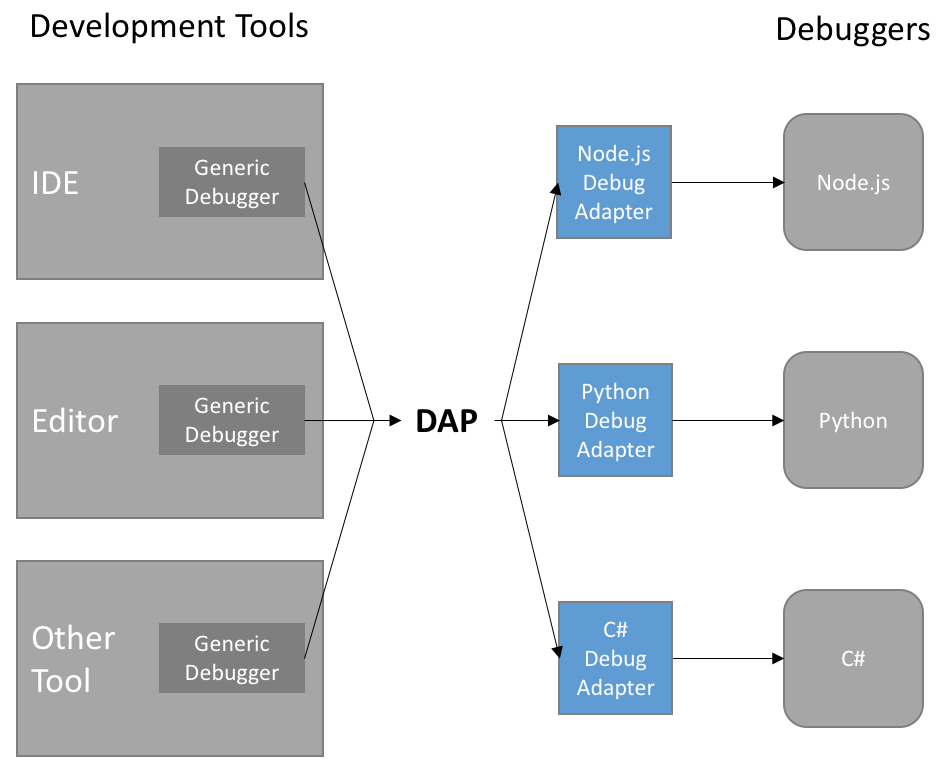
\includegraphics[scale=0.35]{debug-arch.png}
                        }{\tiny{\textcopyright{Microsoft Corporation. https://vscode.readthedocs.io/en/latest/extensions/example-debuggers/}}}
                        \caption{Diagram displaying the relationship between Editors and Tools, the Debug Adapter Protocol, Debug Adapters and the possible Debug Runtimes. Not shown are the
                            editor/tool dependent shims. Each \textit{Development Tool} contains a debugging utility that speaks the Debug Adapter Protocol to communicate with various Debug
                            Adapters.}
                        \label{fig:debug-arch}
                    \end{figure}

                \subsubsection{Concept}
                    Conceptually, the role of the debug adapter created for this project is simple: given a trace ID, it should fetch the spans and their metadata for the trace ID, load the 
                    source code files for each span and allow the user to step through the code on a span-by-span basis (or more granular). If successful, the user would be able to see the
                    source code file and line in which the current span was started and step back and forth between spans and their respective source code files and lines. Given the focus
                    around non-monorepo codebases, it should also have the ability to jump to and from files outside the currently opened codebase, assuming that the codebases for the other 
                    services also reside on the user's machine.
                    
                    The main approach to making this set of requirements possible is by utilizing the tag constructs defined in the OpenTracing specification to carry additional runtime or
                    compile time information that provides enough information to the debugger runtime. This can be done by implementing shims that wrap OpenTracing trace implementations with
                    methods that add the required information as tags to newly created span instances. When the debugger runtime queries the backend API, it can request an additional field on
                    the span types that the backend GraphQL resolver resolves by transforming the information gathered by the shims into a format more useful to the debugger runtime than the
                    raw collected information. This results in being able to interface with the same GraphQL query as the project idea that follows this part, while not incurring the 
                    transformation costs in the following idea.
                    % TODO: word this better

                    In practice, there are a number of challenges that arise in various parts of this concept; gathering the information required to pinpoint the source file and line varies 
                    in format across different programming languages, amount of stack trace information that is to be or that can be gathered and its formats across different programming 
                    languages, mapping different services to the location in the filesystem of their codebase as well as handling spans emitted from services not appropriately instrumented 
                    for this to work. There are different trade-offs with various approaches to these problems that will be outlined.

                \subsubsection{Collecting and Parsing Runtime Data}
                    When dealing with collecting information on the source file and line number at which a span was started, there are two main approaches with highly contrasting pros and cons.
                    The first approach is to simply query the runtime, where applicable, for the file path and line number associated with the function that invoked the span creation. This is often
                    a relatively cheap operation, with a small footprint in the amount of data that a span is tagged with. The main downside of this approach is that while it results in a small 
                    amount of extra data attached to a span, this reduced amount of information reduces the capabilities of the debugger runtime. With this information, the debugger runtime is
                    limited to jumping between those single, individual points in the code at which the spans are created (this could be expanded to also wrap the log-point calls to do the same).
                    
                    The second approach involves querying the runtime for an entire stacktrace leading up to this point. With this approach, there is considerably more data, with all the function
                    calls of the stack frame tree branch leading up to the span creation being gathered, allowing for the possibility to step back and forth at the function level rather than simply
                    at the span level. In both these instances, the data is attached to spans as tags. This approach was chosen to be explored for the project due to the larger potential that accompanies
                    the greater amount of data. For further processing outlined in the following paragraph, the programming language from which the span originates is added as a tag to the span.
                    There are a few downsides to this approach and possible workarounds that will also be discussed.
                    
                    In many language implementations of the Jaeger tracer, tag values are limited in length to either 256 or 1024 characters. When dealing with stacktraces, this limit is too 
                    restrictive for storing entire stacktraces. This is due to an outstanding issue in Jaeger client implementations when using UDP as the transport protocol, as span sizes
                    would exceed the maximum UDP packet size of 65535 bytes\cite{udptagsize}. This makes using HTTP as the span transport method a hard requirement to avoid UDP packets being
                    dropped, causing entire spans to be lost. The client implementations also provide an interface for changing the max tag value length, which must be utilised to prevent the truncating
                    of the stacktraces. As this number cannot be set on a per-span basis, it must be set at a reasonably large number ahead of time based on previous examples of possible stacktrace sizes
                    or the maximum value of an integer for the given platform. Another downside to full stacktraces is that the procedure for getting an entire stacktrace and transforming them can often 
                    be considerably more expensive than adding simple tags to a span. Unfortunately, sampling rules in the Jaeger client implementations, the processes by which it is decided whether or 
                    not spans are exported, are only applied to log points and the final reporting of spans. This results in the potentially expensive operation of gathering stacktraces to be run even if 
                    the span will never be reported. Despite implementing head-based sampling, where it is know when the root span is created whether or not the trace will be reported, the API does not 
                    expose an interface for querying this fact. For this reason, it was important to make the operation as cheap as possible, leaving as much of the stacktrace transformations as possible to 
                    query time, when the debugger runtime requests a trace from the backend.

                \subsubsection{Interfacing GraphQL API with Debug Adapter}
                    With the stacktrace stored in the database as a span tag in string format, the backend GraphQL schema is amended by adding a field to the span type with an associated resolver and 
                    types that define a stacktrace and its individual stack frames. This resolver reads the stored stacktrace and the programming language associated with the span to process it into a 
                    stacktrace object usable for the debugger runtime. As each language has a different format for its stacktraces, a stacktrace parser must be created for each language supported. These
                    will parse the raw stacktrace strings and returns them as a parsed and formatted stacktrace object to the GraphQL resolver. Listing~\ref{lst:stack} shows the updated GraphQL schema
                    with the unchanged sections filtered out. 

                \bigskip
                \begin{lstlisting}[caption={GraphQL schema updated with stack- trace and frame objects. Unchanged fields and objects filtered. The \texttt{shouldReslolve} field indicates
                    whether a file path requires additional resolving in the debugger runtime.}, language=GraphQL, gobble=20, label={lst:stack}]
                    type Span {
                        // ...
                        stacktrace: StackTrace
                    }

                    // ...

                    type StackTrace {
                        stackFrames: [StackFrame!]!
                    }

                    type StackFrame {
                        packageName: String
                        filename: String!
                        line: Int!
                        shouldResolve: Boolean!
                    }
                \end{lstlisting}
                \bigskip

                In this format, the debugger runtime has a more language agnostic representation of the stacktraces collected over the lifetime of a trace. There are still differences
                in how absolute local paths are resolved from this information in order to load the correct file in the editor from the users local filesystem, from differences in how
                codebases are structured into different packages for encapsulation and modularisation, as well as where dependencies are stored in the filesystem. For simplicity, 
                resolving dependencies was not included in this project outside of the standard library for languages where implementation was trivial.

                Alongside showing a stacktrace and the line in the file where the current span was created (or in the case of traditional debuggers, the line it has halted execution on),
                editors often have a panel dedicated for displaying local and global variables for the current stack frame and execution context. Largely due to performance reasons, it is
                not possible to attain this level of information on local and global variables when in the distributed tracing context unlike when using a halting debugger, assuming that 
                \textit{DWARF} symbols (\textit{Debugging With Arbitrary Record Formats}, a standardized debugging data format embedded in executable binaries)\cite{dwarf} are still baked 
                into the binary, which may not always be the case, as it is not uncommon for binaries to be stripped of DWARF symbols to reduce their size. Instead of this, the different types off
                tags and other key-value pairs can be displayed in said panel in place of variables. This works best when traces are heavily tagged with rich, high cardinality metadata which gives 
                greater insight into a service's behaviour, both through the debugger interface and other means, and larger dimensionality with which to reduce a set of traces down to those with 
                a common set of tags that exhibit certain behaviour.
                % TODO: is this the right place for that last line? why else would we want high cardinality 

            \subsection{Service Topology Frontend}
                In the service topology part of the project, the aim is to explore how to increase the value derivable from graph representations of the topology of a service architecture, at 
                both an individual trace level and in aggregate. A common visualisation in many vendors in basic formats, they are commonly based on a type of directed graph called a 
                \textit{force-directed graph} due to its aesthetically pleasing properties. In the following section, the two main classes of service topology visualisations will be introduced,
                monitoring oriented and metrics based visualisation as well as observability oriented and event based visualisations, with the differences between the two being highlighted with an 
                emphasis on the need for the latter type.
        
                A basic service topology graph can give a quick overview of the dependencies between different services in a distributed system. However, it provides little value as an observability tool
                for debugging production issues or finding internal services that are returning errors for certain customers. For developers and administrators to derive tangible value from such a 
                visualisation, there is a need for a more dynamic system. The ability to generate views based on arbitrary attributes would allow for users of the system to create more personalized and 
                focused graphs based on their needs, such as grouping by high cardinality fields like end-user IP address, user identifiers as well as metrics such as error rates, response times 
                etc\cite{doingitwrongtopo}.

                While they are commonly found in distributed tracing vendor services, the implementations are often very simplistic. A common example of such an implementation begins with a basic, often directed
                graph of each service as defined by the service name metadata passed into a tracer implementation. From this, the relationships between graph nodes is drawn by querying a spans service name
                and that of its parent span, which gives both the relationship and the directionality of said relationship. Nodes and edges are then often annotated with various metrics derived from the various
                span fields and tags, with average or percentiles of span durations as well as error rates and number of requests per unit of time being the standard figures on display. Figure~\ref{fig:risingstacktopo}
                is an example of such an implementation from The RisingStack's NodeJS monitoring platform. Often misrepresented as features of \textit{observability} platforms or services, graphs of such kind are
                more aptly described as features of \textit{monitoring} platforms or services. The line between the two terms is often intentionally blurred by vendors which provide monitoring services looking to sell
                to companies who are in need of observability services. Monitoring is commonly described as being how \textbf{known-unknowns} are handled, including defining thresholds for values on metrics such as
                error rates or response times, most commonly working with pre-aggregated data of low dimensionality to give a quick, overview of the system in aggregate. Such systems are ideally tailored towards 
                answering the questions one knows to ask beforehand, hence known-unknowns, which can range from questions such as does the database server require more CPU power or if a recent deployment of a service
                was correlated with an increase in API errors. 

                \begin{figure}[hbt!]
                    \centering
                    \copyrightbox[r]{
                        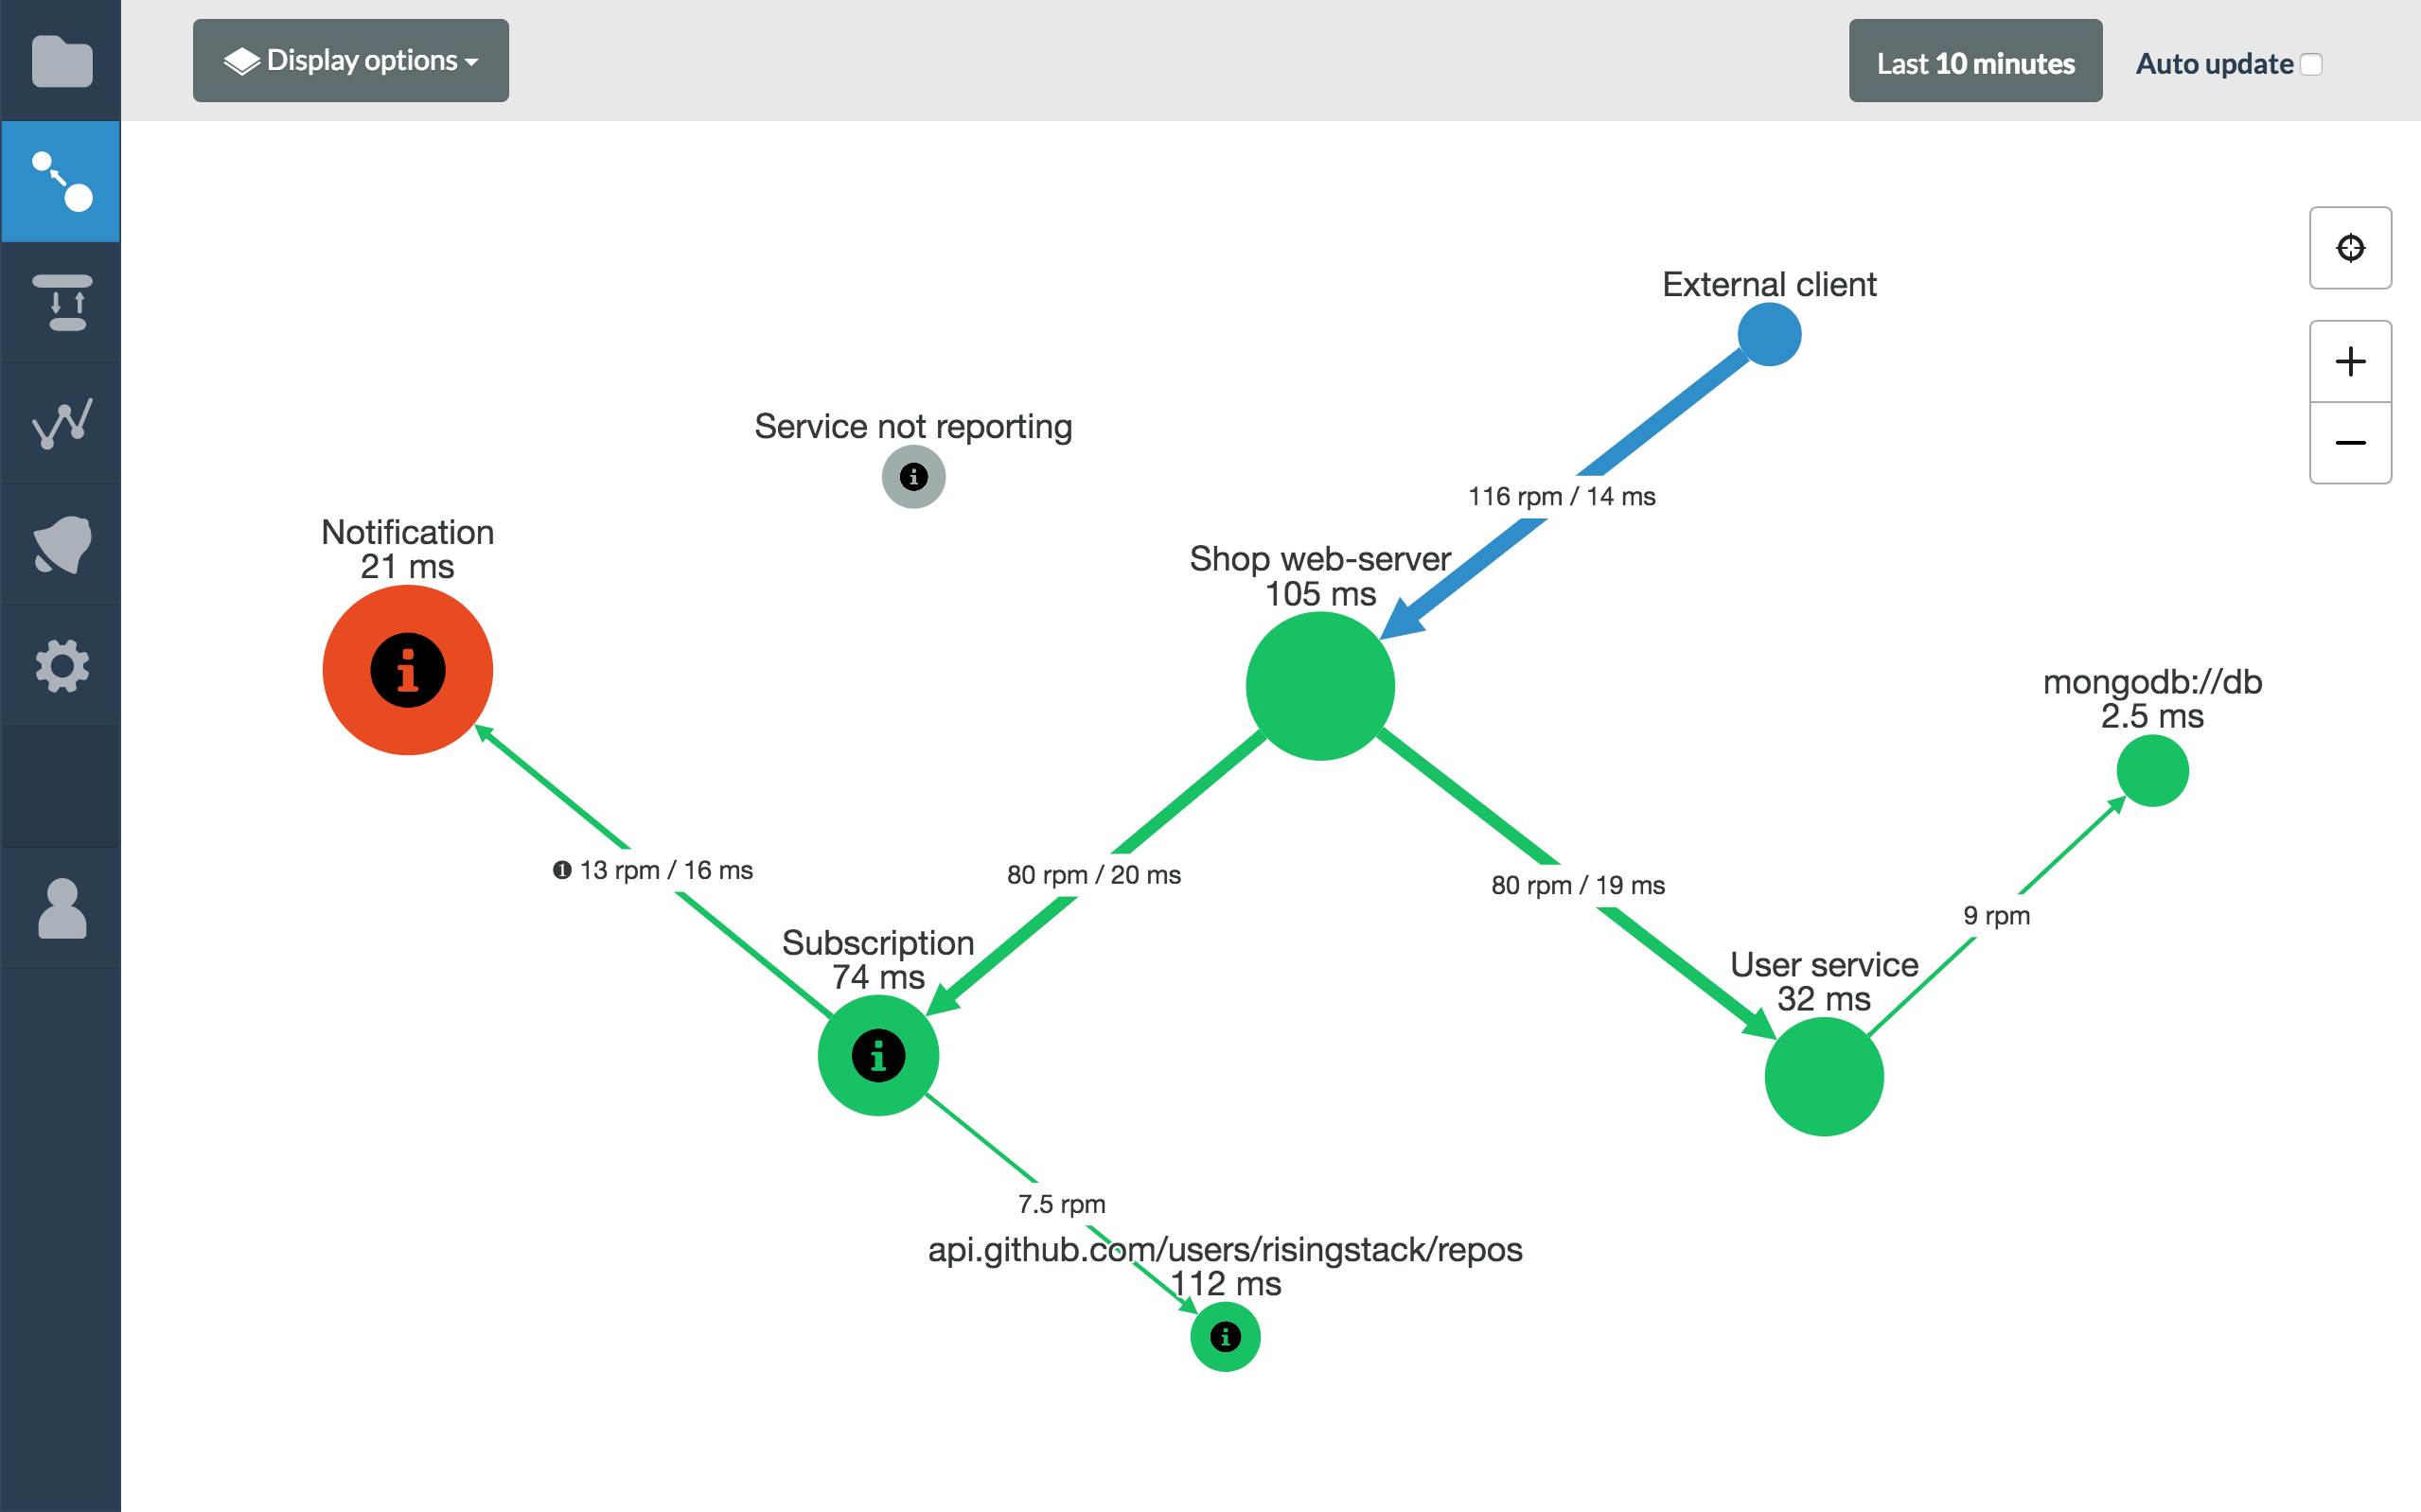
\includegraphics[scale=0.14]{service-topo-risingstack.png}
                    }{\tiny\textcopyright{Gergely Nemeth on The RisingStack blog. https://blog.risingstack.com/distributed-transaction-tracing-microservices-monitoring/}}
                    \caption{Example of the Microservices Topology visualisation from RisingStack's monitoring platform, showing a basic topology overview with key metrics based on traces.}
                    \label{fig:risingstacktopo}
                \end{figure}

                In contrast, observability is all about the \textbf{unknown-unknowns}, being able to ask different, unforeseen questions to a highly dimensional dataset with high cardinality fields that allow
                for arbitrary operations on raw, non-aggregated events, with the ability to drill down on individual events in the set from an aggregate overview. This allows one to receive answers to the questions 
                on the behaviour of a system, in arbitrary aggregate down to an individual level. This sets the tone for what an advanced service topology visualisation should provide to allow for it to be distinguished 
                from standard monitoring alternatives. Building off an event-based, non-aggregated dataset, the service topology graph will start out in a similar fashion to the aforementioned metrics based implementations,
                however in contrast deriving metrics at query time from the events. This will serve as the foundation from which additional operations and features will build off.

                \subsubsection{Filtering}
                    The first vital operation that this visualisation should have is the ability to filter out traces from the working dataset arbitrarily. This allows us to reduce the amount of noise affecting the metrics
                    on display at the edges and nodes, giving users the metrics specific to the new, filtered dataset view. As the user filters on various fields of arbitrary cardinality such as specific error codes,
                    company identifiers or even performs filter operations on derived metrics such as the requests to a service with response times above a certain threshold, the metrics displayed on the graph such as HTTP error codes, 
                    response times etc that are displayed in the graph update dynamically to reflect the new working set consisting of the filtered entries from the original dataset, allowing for questions such as "\textit{Is a particular 
                    error associated with any particular service or node?}" or "\textit{What proportion of companies from a certain state with a certain cookie set are experiencing slow response times?}" to be asked without having 
                    instrumented for those particular questions, while being visualised in a service centric style.

                \subsubsection{Grouping}
                    Grouping of data by an arbitrary field is the next operation that provides high value. This operation is a powerful method by which users can discover common traits of events exhibiting certain behaviour as well as the
                    distribution of errors or other field values across events. By virtue of the form of the visualisation, groupings of event objects are displayed inherently by service identifier/name. This trait extends to grouping by
                    additional fields, resulting in groupings always being in conjunction with service identifiers. The outcome of this is a topology view with a node for every service identifier/grouped field value combination. 
                    
                    As an example, assume a small scale service topology of 5 services for a business with 10 customers. The services consist of a database, an API gateway and three internal services. A user sees that the 99th percentile response
                    time between two services, A and B, is abnormally high. To see if this problem is isolated to a specific customer or if it is happening to everyone, they could perform a group operation on the customer identifier. The topology 
                    graph updates, with every service node being multiplied by ten in count e.g. ten nodes for service A, with combinations ranging from \{service name: A, customer ID: 0\} to \{service name: A, customer ID: 9\} and so on, along
                    with the accompanying edges and metrics for each combination. With the response times now separated by customer identifier, the user can see the distribution of the high response times, whether or not it was isolated to 
                    specific customers or not.

                    For the trivial example given, the graph already expands from five nodes to 50 nodes after grouping by customer identifier. For a company with more customers, this would become unwieldy in size and should therefore be used in 
                    conjunction with the aforementioned filtering capabilities to bring the graph down to a manageable size by excluding grouping combinations where the key metrics are not above or below a defined threshold or where a field does not
                    match a given predicate.
                    
                    These capabilities can also be expanded to reduce noise in the case of high cardinality service identifiers e.g. if using a serverless platform such as AWS Lambda in which each serverless function invocation may have a locally
                    unique identifier with a common prefix, the service topology graph may explode with a large number of one-time nodes. A form of conditional grouping, such as grouping all nodes where the service identifier begins with a given prefix, 
                    could vastly reduce the noise from a graph featuring many nodes from ephemeral services as with serverless platforms or in companies with high deployment frequencies where service identifiers are uniquely suffixed on every deployment.
                    
                    % cookie example or 'what do these have in common'

        \newpage          
        \section{Implementations}    
            \subsection{Debug Adapter}
            \label{sec:impldebug}
                The debugger implementation consists of a number of components that together form a whole package that can be used to extend the Visual Studio Code editor to provide users with the ability
                to step through code of the different codebases residing on the users machine that together make up a distributed system. The main implementation details such as interfacing with the backend
                server outlined in Section~\ref{sec:backend}, how the data is consumed and presented to the user will be discussed in this section.

                As both the Debug Adapter Protocol, Visual Studio Code and TypeScript are all maintained by Microsoft, and given that Visual Studio Code is built on TypeScript with comprehensive support for the language
                in developing extensions for it, TypeScript was the obvious choice to implement this project in. Microsoft provide a sample Github repository containing a mock debugger runtime, Visual Studio Code extension
                and debug adapter. As it contains the necessary boilerplate code from which a fully-fledged debugger runtime and debug adapter can be made, it served as the base for this project.

                The debugger is composed primarily of three parts: the extension that Visual Studio Code loads, the debug adapter that the extension initialises and informs Visual Studio Code about, and the debugger runtime
                that consumes distributed tracing data from the GraphQL server and for which the debug adapter acts as a bridge so that Visual Studio Code can communicate with it. With reference to Figure~\ref{fig:vscodedebug},
                the \textit{Debug Extension} is the metadata that defines the extension that Visual Studio Code consumes, which can be found in the \texttt{package.json} manifest file. This includes the entrypoint JavaScript file 
                that starts the extension, what it contributes as an extension (in this case, a debugger) amongst other metadata. Following on from this, the \textit{Extension Code} includes the entrypoint defined in the 
                aforementioned metadata, and handles the activation, deactivation and the registering of its capabilities through the \textit{Extension API}. One such capability that can be registered is a \textit{Debug Adapter 
                Descriptor Factory}. From this factory, a debug adapter can be activated and the information required for Visual Studio Code to interact with the debug adapter, the \textit{Descriptor} part of the previous term, 
                is consumed by Visual Studio Code. This allows Visual Studio Code to interact with the \textit{Debug Adapter} directly over the \textit{Debug Adapter Protocol}, communicating with the \textit{Debugger} through the 
                Debug Adapter.

                \begin{figure}[hbt!]
                    \centering
                    \copyrightbox[r]{
                        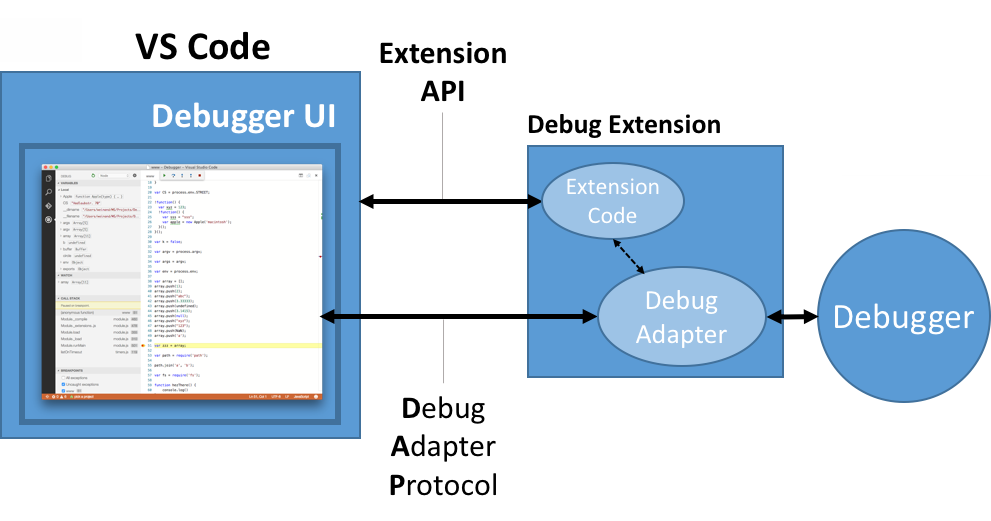
\includegraphics[scale=0.37]{vscodeadapter.png}
                        }{\tiny{\textcopyright{Microsoft Corporation. https://vscode.readthedocs.io/en/latest/extensions/example-debuggers/}}}
                        \caption{The relationships between Visual Studio Code, the Extension API, the Debug Adapter Protocol, the Visual Studio Code extension, the Debug Adapter and the Debugger Runtime in allowing
                        Visual Studio Code to interact with arbitrary debuggers through a common protocol.}
                        \label{fig:vscodedebug}
                    \end{figure}

                \newpage
                Visual Studio Code provides two main types of Debug Adapter Descriptors that define how the debug adapter is run and interacted with: a socket based server or an executable. As this debug extension is wholly self contained, 
                (all three components, the extension, debug adapter and debugger runtime, are part of a single NodeJS compilation unit) the descriptor type chosen was the socket based server. Upon initialisation, a socket based server is 
                created that creates an instance of the debug adapter class when a connection is made. Once the socket is ready to accept connections, Visual Studio Code is informed of the port that it is listening to, so that Visual Studio 
                Code may interact with it. Listing~\ref{lst:descriptor} highlights the basic code required for declaring a method for creating a socket-based debug adapter descriptor. An instance of the \texttt{AdapterDescriptorFactory} class 
                is registered with Visual Studio Code by the extension under a given name. This instructs Visual Studio Code on which debug adapter descriptor factory to invoke the \texttt{createDebugAdapterDescriptor} method on in order to 
                initialise a debug adapter instance to communicate with.

                \newpage
                \begin{spacing}{1.0}
                    \begin{lstlisting}[label={lst:descriptor}, gobble=24, language=TypeScript, caption={The method used to initialise the Debug Adapter and return the Debug Adapter Descriptor to Visual Studio Code.}]
                        class AdapterDescriptorFactory implements DebugAdapterDescriptorFactory {
                            
                            createDebugAdapterDescriptor(
                                session: DebugSession,
                                executable: DebugAdapterExecutable | undefined
                            ): ProviderResult<DebugAdapterDescriptor> {
                                const server = Net.createServer(socket => {
                                    const debugAdapter = new DebugAdapter()
                                    debugAdapter.setRunAsServer(true)
                                    debugAdapter.start(socket, socket)
                                }).listen(0)

                                return new vscode.DebugAdapterServer(
                                    (this.server.address() as Net.AddressInfo).port
                                )
                            }
                        }
                    \end{lstlisting}
                \end{spacing}

                The debug adapter and debugger runtime communicate in an asynchronous fashion through regular method invocations. Upon initialisation, the debug adapter also initialises an instance of the debugger runtime, adds an event handler 
                on it to listen for emitted events from the debugger runtime and saves a reference to the initialised object. The debug adapter is then ready to receive events from Visual Studio Code, upon which it receives the \textit{Initialize}
                request, in which the client (Visual Studio Code in this instance) and debug adapter inform each other of their capabilities according to the debug adapter protocol specification, the \textit{Configuration Done} request, which informs 
                the debug adapter that the client has finished initialisation, and finally the \textit{Launch} request. For a visual representation of a more exhaustive flow given a richer set of capabilities announced by the debug adapter than were
                included in the scope of implementing this final year project, see Figure~\ref{fig:dapflow}, with the full specification and overview available online at \url{https://microsoft.github.io/debug-adapter-protocol/specification}.
                
                \begin{figure}[htb!]
                    \centering
                    \copyrightbox[r]{
                        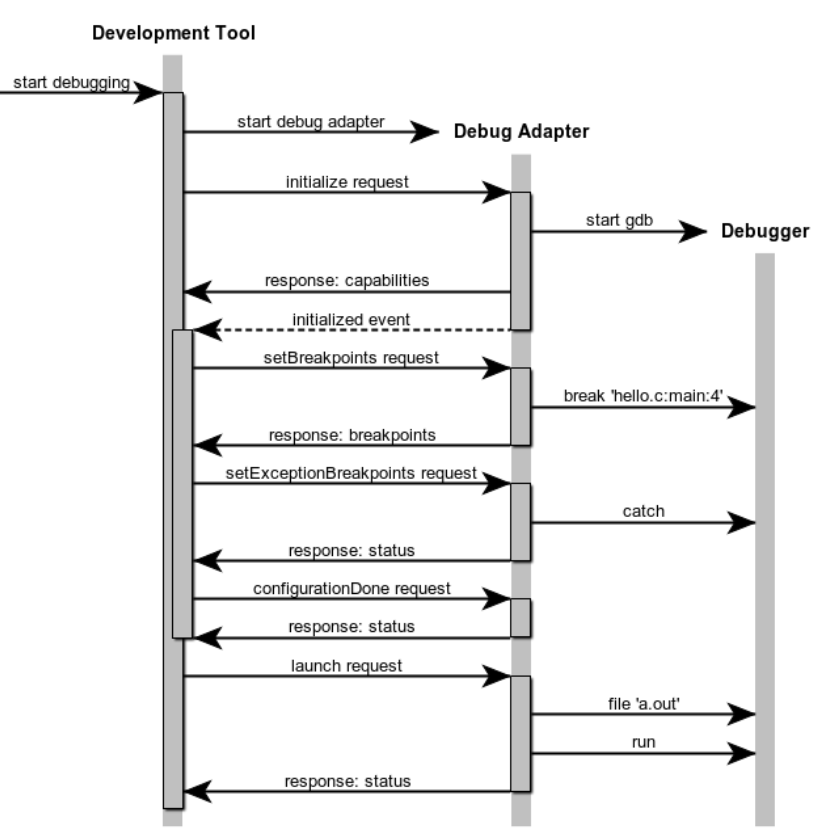
\includegraphics[scale=0.4]{dapflow.png}
                    }{\tiny\textcopyright{Microsoft Corporation. https://microsoft.github.io/debug-adapter-protocol/overview}}
                    \caption{The diagram illustrates the order of events and requests communicated between the a tool such as Visual Studio Code, a Debug Adapter and the Debugger Runtime that the Debug Adapter wraps.}
                    \label{fig:dapflow}
                \end{figure}
                
                When the debug adapter receives a request from Visual Studio Code to perform a certain operation such as step forward or backwards, it invokes the relevant method on the debugger runtime and sends a \texttt{success} response back
                to Visual Studio Code if the method call was successful. The debugger runtime in turn can notify the debug adapter of specific events that it emits after a method was called on it such as when it halts on a line, when it terminates 
                etc. The debug adapter then creates the associated Debug Adapter Protocol event type and sends said event to Visual Studio Code to handle.

                \newpage
                Execution of the debugger runtime at a high-level involves only a small number of basic operations. The majority of the complexity comes about from the bookkeeping of a number of values and how they change as the user steps 
                through code of numerous files throughout their machine; a mapping of service names to local filesystem paths that is updated as new services are encountered while stepping through files, persisting new values as they are input
                by the user; a set of append-only arrays that are initialised from the stack frames of the first span when the debugger runtime starts execution; and a single integer variable that keeps track of where in these arrays the debugger
                runtime is currently halted on. The append-only arrays consist of: an array of filepaths which are resolved to their local path on the user's machine, an array of stack frames and an array of span index numbers that associate a stack 
                frame in the previous array with the index of the span in the list of spans the trace holds that the stack frame was associated with. As these three arrays are always the same length, the array-tracking index variable gives convenient
                access to the currently active stack frame, span and file path. This allows for the ability to step forwards as well as backwards through the stack frames, while always having the relevant span and file info available, greatly 
                simplifying the process of displaying the tags of the currently active span.
                
                On each step-forward request, the debugger runtime checks if the next span's data must be loaded into the append-only arrays by checking if the array-tracking index has reached the end of the arrays, loading data the same way
                as the first span was, as mentioned previously. Span and stack frame data is lazily loaded in this manner until all span and stack frame data has been loaded into the arrays, ensuring that user input that may be necessary to resolve
                some filepaths is not requested upfront for every stack frame stored in the spans of a trace. Once the list of spans has been exhausted, the user is simply informed of such in a notification. For step-back requests, the process is
                considerably simpler. As the data is already loaded, there is no need to load anything additionally. The array-tracking index is decremented instead of incremented, until such point as it hits zero when the first stack frame from the
                first span has been reached.

                As the debugger runtime steps through each stack frame one by one, it notifies the debug adapter to emit a \textit{Stopped} event for each one. This indicates that the debugger runtime has stopped execution, with an accompanying reason 
                as an attribute on the event that can be of a value such as "step", "breakpoint", "exception" etc. In this case, only the "step" reason is used, as the debugger runtime stops walking the stack frames on every individual step. Every time
                this event is received by Visual Studio Code, a number of requests are made to the debug adapter: a \textit{Threads} request that fetches a list of threads that exist at this point in time, a \textit{StackTrace} request that returns
                a stacktrace for the given thread identifier that is associated with a \textit{Stopped} event, a \textit{Scopes} request that fetches the set of variable scopes such as global and local scopes in the case of more traditional debugger
                environments, and finally a \textit{Variables} request for every scope defined in the previous request. Of particular interest are the \textit{Scopes} and \textit{Variables} requests. Through these request, it is possible to provide a 
                set of variables to be displayed in the debugger UI, grouped by a defined scope. In the context of distributed tracing, with Jaeger in particular, there are three notable groups of data that can be easily transformed into the role of
                variable scopes; the span tags, the process tags (tags assigned to a particular tracer) and baggage items (data that is carried across process boundaries in the span context). These can each be defined as a debug adapter protocol scope,
                and the set of values in each can become the set of debug adapter protocol variables for each. Figure~\ref{fig:scopes} shows an example of how this would look in the Visual Studio Code debugger UI, with the three scopes being expandable
                to display the set of variables for each. 

                \bigskip
                \begin{figure}[htb!]
                    \centering
                    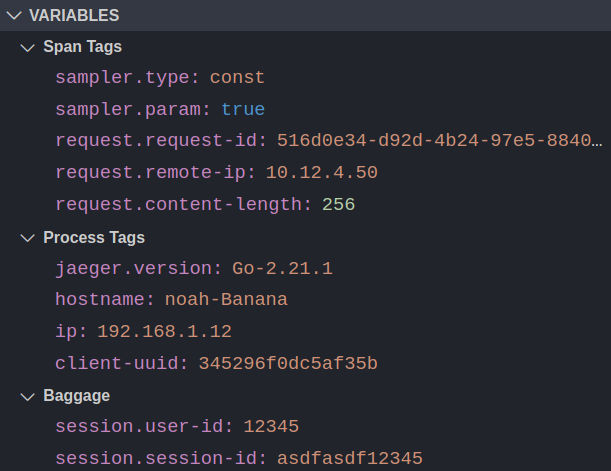
\includegraphics[scale=1.7]{scopes.png}
                    \caption{The Variables view in the Visual Studio Code debugger UI, displaying three named variable scopes with expandable menus to show or hide the variables
                    in each scope.}
                    \label{fig:scopes}
                \end{figure}

                In a similar fashion, the \textit{StackTrace} request can be used to show a list of stack frames leading up to the current active stack frame in a separate panel in the Visual Studio Code debugger UI. While the extent of 
                features available from this representation is dependent on the editor or tool in question, in the context of Visual Studio Code, it allows for users to click on individual stack frames and be immediately transported 
                to the source file and line associated with the clicked stack frame, without losing sight the current active stack frame, being able to trivially return to it by clicking on it in the UI. Figure~\ref{fig:stacks} shows a 
                sample of how this would look in Visual Studio Code, with information displayed such as the service, span name, source file and line for each stack frame.

                \begin{figure}[htb!]
                    \centering
                    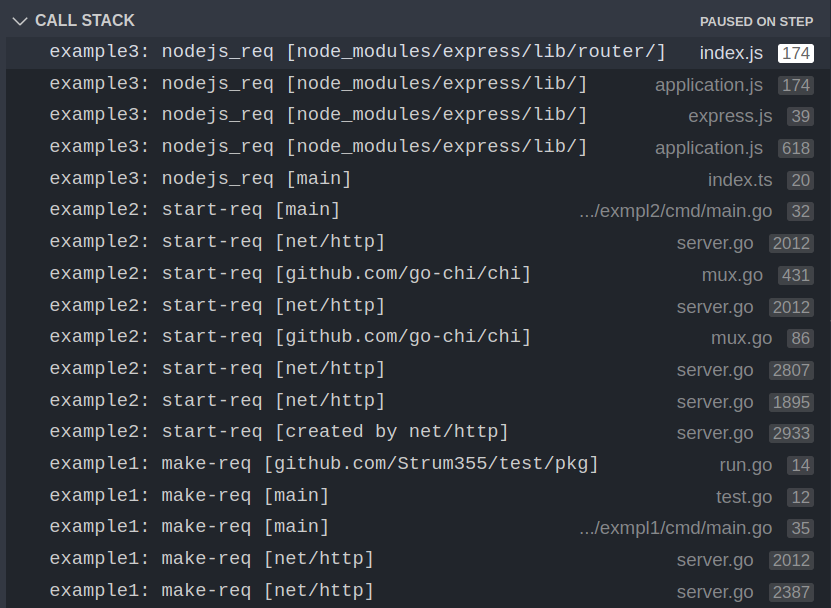
\includegraphics[scale=1.6]{vscodestack.png}
                    \caption{The visualisation of stack frames in the Visual Studio Code debugger UI panel, displaying various information such as the service name, operation/span
                    name as well as source file information for each stack frame, displayed in a top-down manner.}
                    \label{fig:stacks}
                \end{figure}

                \newpage
                The Debug Adapter Protocol provides a rich specification for providing debugger runtime agnostic debugging capabilities that allows for a comprehensive set of features to be implemented in a vast range of environments.
                It was fundamental in allowing for highly multi-editor compatible debug adapter and debugger runtime implementations that utilise OpenTracing distributed tracing data to provide a debugging experience that feels similar
                to using a traditional debugger such as gdb or delve in a non-blocking manner. However, the data required to provide such capabilities must be generated and collected at runtime by the individual services. The next section
                will describe how this was implemented for the programming languages implemented, as well as attempts made during development that fell short of providing an optimal solution.

                % baggage, tags, process tags, libraries, 

            \subsection{OpenTracing Tracer Shims}
                As the debugger runtime and backend API server rely on runtime stacktrace information in order to step through stack frames for each span in a trace, the instrumented services need to be able
                to collect that information as well as any other information required for operations such as dependency path resolution and transport it to the trace collector as part of the span tags.
                To achieve this, a lightweight shim that implements the OpenTracing tracer API was implemented for every language supported. A number of languages were originally considered and then narrowed
                down to a set that were found to be viably implemented. Originally considered were: NodeJS with which comes support for TypeScript, JavaScript, CoffeeScript and other languages that compile
                down to JavaScript, Go, the JVM including Java and Kotlin, Python and Rust. This was narrowed down to NodeJS, Go and the JVM.

                \subsubsection{NodeJS Tracer Shim}
                    The NodeJS OpenTracing tracer shim implementation was made simple by the constructs made available by the NodeJS runtime to gather much of the required information easily. As each \texttt{Error} 
                    instance has a stacktrace attached with it, gathering a stacktrace is as simple as referencing the \texttt{stack} attribute. By default however, the stacktrace is limited to ~10 entries. This is
                    easily remediated, by setting the \texttt{stackTraceLimit} static attribute on the \texttt{Error} class to \texttt{Infinity}, ensuring the full stack trace possible.

                    However, there were some scenarios in which the full stacktrace would not be captured. Due to how NodeJS handles asynchronous execution of functions\cite{asyncnostack}, there are scenarios in which
                    the stacktrace context is lost. While there have been solutions released to try alleviate this issue, including natively in the NodeJS runtime\cite{asyncstack}, there still remains scenarios in which
                    the stacktrace is substantially smaller with much context lost. The \textit{trace}\cite{longtrace} NodeJS package was discovered that showed good results in the sample NodeJS microservice codebase, and was
                    integrated into the shim thereafter.

                    Figure~\ref{fig:nodejsstack} illustrates an example of a NodeJS stacktrace as it is stored in the database. Of note is the absolute filepath on every line. As the filepath associated with a stack
                    frame is vital, it is necessary to derive the paths relative to the path of the main module so that it can be resolved properly to the location of the file on the end user's machine. For this, the 
                    shim queries the NodeJS runtime for the filepath of the entrypoint script and deriving the directory it is contained in via the following snippet: \texttt{require('path').dirname(require.main.filename)}.

                    As JavaScript is increasingly not being used directly by developers, but rather through languages such as TypeScript, CoffeeScript, Elm and other programming languages that transpile to JavaScript,
                    as well as the fact that JavaScript is commonly transformed and minified for more efficient browser delivery, the concept of \textit{source mapping} was created to map stacktrace information
                    from the transformed sources to the original source code. While NodeJS supports displaying associated source mappings alongside the transformed source filepaths in stacktraces\cite{sourcemap},
                    the \textit{source-map-support}\cite{sourcemapsupport} NodeJS package takes this further by replacing the transformed source filepaths with the original source mapping filepaths, "making every 
                    compile-to-JS language more of a first-class citizen", making first-class citizens of languages that compile to JavaScript in the stacktraces simplifies the processing needed on the backend, 
                    outlined in Section~\ref{sec:backend}.

                    \begin{figure}[hbt!]
                        \centering
                        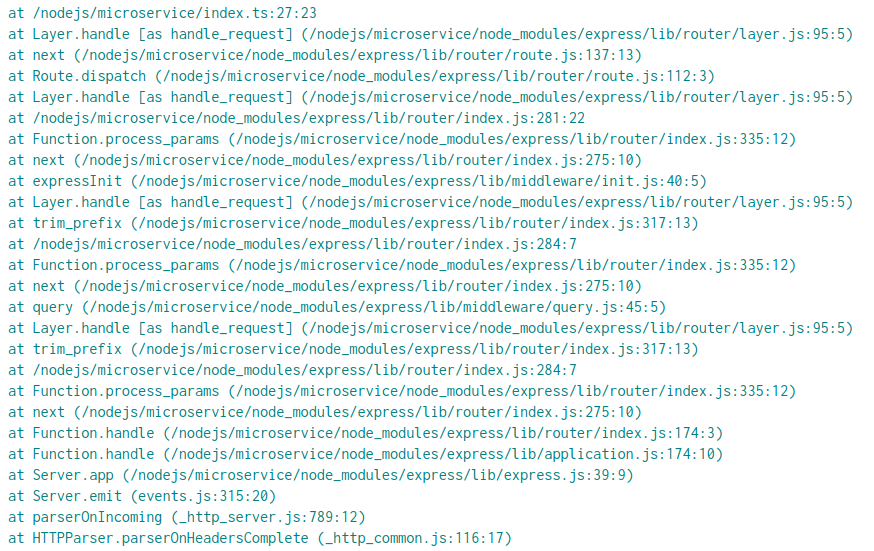
\includegraphics[scale=1.7]{nodejsstack.png}
                        \caption{NodeJS stacktrace collected in a HTTP handler on processing an incoming request with the Express HTTP framework for JavaScript.}
                        \label{fig:nodejsstack}
                    \end{figure}

                    In whole, the NodeJS shim attaches three tags to every span created through it: the stacktrace string to be parsed by the backend API server, the language/platform (namely "nodejs"), as well
                    as the full directory path of the entrypoint of the application, as this is required to in the backend API server to trim the filepath prefixes to allow for resolving to the application
                    root directory on the end user's machine. Next the Go tracer shim implementation will be discussed, along with the differences encountered compared to the NodeJS tracer shim.

                \subsubsection{Go Tracer Shim}
                    The Go tracer shim implementation came along with a wholly different set of problems to solve. As with NodeJS, capturing a stacktrace in Go is made trivial by the Go standard library. However,
                    in a similar fashion, the stacktrace returned by the Go runtime does not go further than the point where a function was called as a goroutine\cite{goroutine}, the term used in Go to refer to a 
                    form of green threads employed by the language to achieve concurrency. In contrast to NodeJS, this behaviour is consistent for all tested scenarios, which establishes confidence in the quality 
                    of the returned stacktrace. Figure~\ref{fig:gostack} displays a stacktrace collected in Go, which will be described in more detail in Section~\ref{sec:goparser}. Of particular note, in the context
                    of stacktraces collection in asynchronous contexts, are the final two lines of the stacktrace, where the indication is made that this stack frame is the beginning of a new goroutine ("\texttt{created
                    by net/http.(*Server).Serve}"), with the function name, source code path and file line number of the function that created the goroutine outlined.

                    \begin{figure}[hbt!]
                        \centering
                        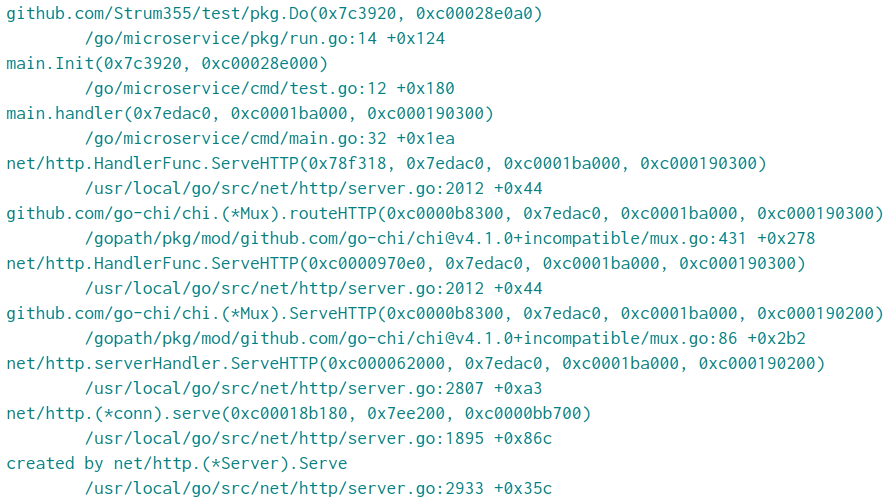
\includegraphics[scale=0.4]{gostack.png}
                        \caption{Go stacktrace collected after two functions calls from within a HTTP handler.}
                        \label{fig:gostack}
                    \end{figure}

                    While in the NodeJS tracer shim, it was possible to query for the directory path of the project root directory, this proved to not be a portable solution for the Go implementation. The filepaths
                    in the stacktrace are based off compile-time values, therefore using the runtime project root directory would yield a value that cannot be applied to the trimming the filepaths in the stacktrace. 
                    After researching methods for retrieving the value of the compile-time project root directory, the most optimal solution that was found was to utilise compiler linker flags to set values at compile
                    time\cite{golangldflag}. By invoking the compiler as follows, it is possible to set the value of the project root directory variable at compile time: '\texttt{go build -ldflags "-X 
                    github.com/Strum355/tracestep/golang.GoModulePath="\$(pwd) cmd/*.go}'. \\The Go tracer shim adds one extra tag to each of its spans compared to the NodeJS tracer shim, a value to represent the 
                    \texttt{GOPATH} environment variable at compile-time. Unlike in NodeJS, dependencies are commonly stored in a central directory in the filesystem, and as such to resolve them, said directory needs to
                    be known to mark the relevant stack frames as requiring extra resolving, either via user input or by looking up a previously stored value for the value of \texttt{GOPATH} on the end user's machine,
                    when consumed by the debug extension in Section~\ref{sec:impldebug}. All other processing is then handled by the backend API server for the debug extension to consumes, which will be discussed in the 
                    following section.

                
                % TODO: GET IT DONE. The Python Jaeger client libraries did not support transporting spans over HTTP, with only UDP transport support. 
                % TODO: GET JVM DONE TOO
                % go and node, python bad coz UDP, https://golang.org/cmd/link/

            \subsection{Backend API}
            \label{sec:backend}
                The backend provides a client- and database-agnostic interface to consume distributed tracing data from the data store. It implements a GraphQL server that allows for the extra computation
                required for some data object attributes to be avoided where not necessary. The main constructs of the backend will be discussed are the GraphQL schema, schema builder and resolver, the stack
                parsers that transform the stacktraces emitted by the tracer shims, how interfacing with the Elasticsearch database was handled, and finally any major issues that were encountered during development.

                It was decided that it would be implemented in Kotlin after evaluating the different Elasticsearch and GraphQL libraries available, of which there were libraries 
                that utilized the Kotlin type-safe builder constructs\cite{dsl} to declare GraphQL schemas and Elasticsearch queries in the Kotlin-based \textit{Domain Specific Language} (DSL), allowing
                for more expressive construction of the GraphQL schema and Elasticsearch queries natively in the language. 
                
                Listing~\ref{lst:kgraphql} illustrates how the GraphQL schema is defined in Kotlin code. The GraphQL Kotlin implementation is maintained by Jógvan Olsen, and can be found at 
                \url{https://github.com/aPureBase/KGraphQL}. Line 2 defines a field on the Query top-level object, an entrypoint into the server named \textit{"findTrace"} that takes a single string parameter 
                denoting the trace identifier of the trace object that is being requested. This identifier is passed to the data storage repository instance, of which there is only a simple Elasticsearch 
                repository implemented. Additional data stores such as Apache Cassandra are not implemented, however they may be trivially implemented as the GraphQL resolver operates on a generic data store 
                interface which abstracts the data storage layer from the GraphQL resolvers.

                Additionally, an extra property is defined on the \textit{Span} type, named \textit{"stacktrace"} for denoting the stacktrace object consumed by the debugger runtime from Section~\ref{sec:impldebug}, 
                and the \textit{"logs"} field already defined on the \textit{Span} type, with a custom resolver to optionally filter the data in the field before the data is serialized. Each custom field resolver takes
                the parent object as the first parameter, upon which further operations are carried out. The stacktrace resolvers purpose is to transform the raw stacktrace stored in the span tag into a defined and common
                format. It does this by reading both the stacktrace and the programming language that this span originated from and processes the stacktrace with the appropriate stacktrace parser, for which there is one
                for every language supported. As two OpenTracing tracer shims were created, one for the Go programming language and one for NodeJS (for JavaScript/TypeScript), two stacktrace parsers needed to be implemented 
                to parse the respective stacktraces into a common format.

                \begin{spacing}{1.0}
                    \begin{lstlisting}[caption=Kotlin snippet of defining the GraphQL schema using the Kotlin DSL., language=Kotlin, gobble=24, label={lst:kgraphql}]
                        val schema = KGraphQL.schema { 
                            query("findTrace") { 
                                resolver { traceID: String ->
                                    // ...
                                }.withArgs { 
                                    arg<String> { name = "traceID"}
                                }
                            }

                            type<Span> {
                                property<StackTrace>("stacktrace") { 
                                    resolver { span ->
                                        // ...
                                    }
                                }

                                property<List<LogPoint>?>("logs") {
                                    resolver { span: Span, eventType: String? ->
                                        // ...
                                    }
                                }
                            }
                        }                
                    \end{lstlisting}
                \end{spacing}

                \subsubsection{NodeJS Stacktrace Parser}
                \label{sec:nodeparser}
                    In Listing~\ref{lst:nodeparser}, the NodeJS stack parser is illustrated. A sample NodeJS stacktrace is provided in Figure~\ref{fig:nodejsstack} to illustrate the
                    format the parser deals with. A Regular Expression is used to extract the file path and line number for each line
                    in the stacktrace, which is in the format of \texttt{/file/path:line}. The final number in each line denotes the column in the file. This information is not 
                    used for simplicity purposes and to keep a more common stacktrace format, as this information is not present in many languages, however, future endeavours could
                    explore how to utilise it where present.
                    
                    As NodeJS dependencies reside under a common directory in the project directory, path resolving for files of dependencies referenced in the stacktrace is trivial. 
                    Figure~\ref{fig:nodejsstack} shows many stack frames originating from functions in files under the path \texttt{/nodejs/microservice/node\_modules/express}. \textit{Express},
                    a NodeJS HTTP framework, is a dependency of the sample NodeJS microservice, and resides in a subdirectory of the microservice directory, the directory being \texttt{/nodejs/microservice}
                    in the given stacktrace. For this reason, \texttt{null} is passed to the \textit{StackFrame} constructor as the first argument, which denotes the package name to aid in
                    dependency resolution and isolation, as it is not needed for the aforementioned reason.

                    \hl{Earlier in development, before the \textit{clarify}{\cite{clarify}} NodeJS package had been discovered, stacktraces would contain a number of entries that were associated with NodeJS internal 
                    runtime files. The parser was setup to ignore such lines by returning \texttt{null} from the \texttt{mapNotNull} function, which excludes null values from the final list. They were considered unimportant 
                    enough to warrant not being included, as implementing support for language internals is outside of the scope of this project where implementation is non-trivial. As this was no longer an issue
                    after discovery of the aforementioned package, the parser remained unchanged as there was no reason to change it.}

                    \begin{spacing}{1.0}
                        \begin{lstlisting}[language=Kotlin, gobble=28, label={lst:nodeparser}, caption={The NodeJS Stack parser class }]
                            private val scrubber = Regex(""".*?(\/.+?:\d+).*""")

                            class NodeJSStackParser(var stacktrace: String, val execPath: String) {
                                fun parse(): StackTrace {
                                    val seq = stacktrace.split("\n").mapNotNull {
                                        val match = scrubber.find(it)
                                        // the full filepath + line string, early return if no match
                                        val fileInfo = match?.component1() ?: return@mapNotNull null
                                        val (path, line) = fileInfo.split(":")
                                        val strippedPath = path.removePrefix(execPath+"/")
                                        val lineInt = line.toInt()
                                        StackFrame(packageName, strippedPath, lineInt, false)
                                    }
                                    return StackTrace(seq)
                                }
                                
                                private fun extractModule(filepath: String): String {
                                    val pathWithoutFile = filepath.removeSuffix(File(filepath).name)
                                    return when(pathWithoutFile.length) {
                                        0 -> "main"
                                        else -> pathWithoutFile
                                    }
                            }
                        \end{lstlisting}
                    \end{spacing}

                    As the NodeJS OpenTracing tracer shim initialises the \texttt{source-map-support} library, stack frame lines in the stacktrace that have an 
                    accompanying line representing the source mapping are overwritten with the source mapping. This greatly simplifies the stacktrace parsing, as there is only one line
                    associated with each stack frame, with the source mapping being the definitive line where available.
                    % TODO: expand? 

                \subsubsection{Go Stacktrace Parser}
                \label{sec:goparser}
                    Following on from the NodeJS stack parser is the Go stack parser in Listing~\ref{lst:goparser}. Parsing Go stacktraces is notably more involved than parsing NodeJS 
                    stacktraces. Each stack frame is represented by two lines in the stacktrace string: the first line contains the package name, function name and the function call argument 
                    addresses for each parameter of the function called as well as the address of the returned variable(s), while the second line contains the path of the file containing the 
                    function the stack frame represents at compile time, the line in the file and finally program counter information. 

                    The parser initially removes unused data from the stacktrace string, removing the program counter information, function argument and return variable addresses. What remains
                    are the package names with function names and file paths with line numbers on alternating lines. The package names, file paths and line numbers are extracted from this, and
                    as the function names are not needed, they are discarded. 

                    There are five main types of packages that need to be handled in Go: the main package which contains the entrypoint into the application, subpackages of the application,
                    internal packages that are part of the Go standard library, vendored dependencies and lastly non-vendored dependencies. For the main package, subpackages and vendored
                    dependencies, the filepath handling mentioned in Section~\ref{sec:impldebug}, wherein source code filepaths that have the applications base path as a prefix, are resolved by prefixing
                    them with the user-provided base path of the application's path on the users machine, and their package name is set to null. For non-vendored dependencies, the \texttt{GOPATH} 
                    value provided to the tracer shim at compile time is trimmed from the paths and the package name is parsed and set. Finally, for the Go internal package files, the package name
                    is parsed and the filepath is left untouched.

                    This file path parsing makes a number of assumptions for the sake of simplicity, with not every environment scenario considered part of the scope of what it should handle. Firstly,
                    it assumes that \textit{Go Modules} is the dependency management system employed for the instrumented application. As this is the official system being promoted by the Go core team,
                    it was a natural fit to be supported. The older system without versioning also makes use of the \texttt{GOPATH} environment variable, and could be supported without much extra work,
                    while \textit{Dep} makes use of vendoring, and as such is already supported as a side-effect of the implementation. Lastly, it is assumed that all package names, outside of the internal
                    standard library, are in the format \texttt{domainname.tld/author/package/} with any number of subpackages, as the package name parser assumes a single period character in the name.
                    This was considered sufficient for the proof of concept, while implementing support for package names outside of this constraint was considered outside of the scope of the project.
                    % TODO: expand
                    \medskip
                    \begin{spacing}{1.0}
                        \begin{lstlisting}[language=Kotlin, gobble=28, label={lst:goparser}]
                            private val scrubber1 = Regex("""\(((?:0x[a-f0-9]+, )*0x[a-f0-9]+)?\)\n""")
                            private val scrubber2 = Regex(""" \+0x[0-9a-f]+""")
                            
                            class GolangStackParser(
                                var stacktrace: String,
                                val execPath: String,
                                val gopath: String
                            ) {
                                fun parse(): StackTrace {
                                    stacktrace = scrubber1.replace(stacktrace, "\n")
                                    stacktrace = scrubber2.replace(stacktrace, "")
                                    stacktrace = stacktrace.replace(execPath+"/", "")
                                    stacktrace = stacktrace.replace(gopath, "")
                                    val seq = stacktrace.trim().split("\n").chunked(2).map {
                                        val (packageFunc, fileLine) = it
                                        val (path, line) = parseFileInfo(fileLine) 
                                        val shouldResolve = when(path.startsWith("/pkg/mod")) {
                                            true -> true
                                            false -> shouldResolve(packageFunc, path)
                                        } 
                                        val pkg = parsePackageLine(packageFunc)
                                        StackFrame(pkg, path, line, shouldResolve)
                                    }
                                    return StackTrace(seq)
                                }
                            
                                private fun shouldResolve(packageStr: String, path: String): Boolean {
                                    if (!path.startsWith("/")) return false
                                    val packageFuncSplit = packageStr.split(".")
                                    return !packageFuncSplit.first().contains("/")
                                }
                            
                                private fun parsePackageLine(packageStr: String): String? {
                                    val pkgFuncSplit = packageStr.split(".")
                                    if (pkgFuncSplit.first() == "main") return "main"
                                    if (pkgFuncSplit.first().contains("/")) return pkgFuncSplit.first()

                                    return pkgFuncSplit.take(2).joinToString(separator=".")
                                }
                            
                                private fun parseFileInfo(fileInfo: String): Pair<String, Int> {
                                    val (path, line) = fileInfo.split(":")
                                    return Pair(path.trim(), line.toInt())
                                }
                            }
                        \end{lstlisting}
                    \end{spacing}
                
                \subsubsection{Interfacing With Elasticsearch}
                    As the backend interfaces with an Elasticsearch database, there needs to be a way to build an Elasticsearch query that retrieves a specific trace for a given trace identifier. The Elasticsearch Query DSL
                    is based on JSON, which lends itself elegantly to being represented in the Kotlin DSL. Listing~\ref{lst:eskotlin} illustrates a simple yet complete sample for an Elasticsearch query for a document that
                    represents a trace for a given trace identifier, and how it is represented in the Elasticsearch Query DSL. The query builder DSL is provided by a Kotlin library by Mike Buhot, available at 
                    \url{https://github.com/mbuhot/eskotlin}, and the official Elasticsearch client is used to perform the queries against the database.

                    \bigskip
                    \begin{spacing}{1.0}
                        \begin{lstlisting}[caption={Comparison between Elasticsearch query using Kotlin DSL and the query in its JSON representation, where $\langle$traceID$\rangle$ refers
                            to a variable storing the trace identifier.}, label={lst:eskotlin}, language=Kotlin, gobble=24]
                            // Kotlin DSL
                            val query = term { 
                                "traceID" {
                                    value = <traceID>
                                }
                            }

                            // JSON Representation
                            {
                                "term": {
                                    "traceID": { 
                                        "value": "<traceID>" 
                                    }
                                }
                            }
                        \end{lstlisting}
                    \end{spacing}

                \subsubsection{Issues Encountered}
                    During development with the GraphQL library, there were two major issues that were encountered that stalled progress. These were due to differences in how Kotlin treats the Array type, its
                    relationship to the Java Array primitive type and their APIs in comparison to other array-like collection types, and behaviour of Java Virtual Machine Type Erasure\cite{typeerasure} at runtime respectively.
                    
                    \smallskip
                    In Kotlin and Java, the Array types do not implement the \texttt{Iterable} interface, unlike the \texttt{ArrayList} or \texttt{Vector} classes. Originally, KGraphQL checked whether a type implemented the 
                    Iterable interface, which the majority of collection types do. As Arrays do not implement the interface, they were treated as a standard generic class, which causes an exception to be thrown indicating 
                    that generic types are not supported. the \texttt{Arrays} class provides static methods to wrap an Array type with the \texttt{List} API, which implements the Iterable interface without copying the 
                    underlying array. An issue was opened for this on the Github repository, after which Array support was added through use of the aforementioned static method.

                    The second obstacle revolved around type erasure and casting from the \texttt{Any} type (the root type of the Kotlin class hierarchy, as \texttt{Object} is in Java) to an \texttt{ArrayList}. When fetching data from 
                    Elasticsearch, the returned document is represented as a \texttt{Map<String, Any>}, as each value may be of a different type. When fetching the list of tags from the document map, they are cast to an 
                    \texttt{ArrayList<Tag>?}, as list types are stored in an \texttt{ArrayList} in the document map. This cast is technically successful at runtime, however only partially. Due to type erasure, the cast only 
                    confirms that the cast from \texttt{Any} to \texttt{ArrayList} is valid, which it is. However, instead of being an \texttt{ArrayList} of \texttt{Tag} objects, it contains \texttt{HashMap<Any, Any>}, in which 
                    each attribute of the \texttt{Tag} type is a key in the map. After debugging the issue with the KGraphQL library author, the solution was plainly to extract the values from the map into \texttt{Tag} objects.
            

    \chapter{Evaluation}
        %  Not all languages have runtime info for source file and line num eg C, C++
        % performance

        % trimming common frames

        %  This alone, the ability to filter on metrics and arbitrary fields, is made possible already by storing events in non-aggregated form and deriving metrics dynamically. 
    
    \chapter{Conclusion \& Future}
    % showing multiple stacktraces from spans running at the same time
        \section{Conclusion}

        \section{Future Work}
            \subsection{OpenTelemetry}

    \begin{thebibliography}{69}
        \addcontentsline{toc}{chapter}{Bibliography}    

        \bibitem{retrospective}
        Charity Majors, \textit{Observability - A 3-Year Retrospective.} \\
        The New Stack, 6th Aug 2019 \\
        \url{https://thenewstack.io/observability-a-3-year-retrospective/}

        \bibitem{dapper}
        Benjamin H. Sigelman, Luiz André Barroso, Mike Burrows, Pat Stephenson, Manoj Plakal, Donald Beaver, Saul Jaspan, Chandan Shanbhag, \\
        \textit{Dapper, a Large-Scale Distributed Systems Tracing Infrastructure.} \\
        Google, Inc. 2010 \\
        \url{https://research.google/pubs/pub36356/}

        \bibitem{mbta}
        Mike Barry, Brian Card, \textit{Visualizing MBTA Data.} \\
        10th June 2014, \url{https://mbtaviz.github.io/}

        \bibitem{opentracing}
        Benjamin H. Sigelman (co creator), \textit{The OpenTracing project.} \\
        October 2015, \url{https://opentracing.io/}

        \bibitem{opentelemetry}
        OpenTelemetry Authors, \textit{The OpenTelemetry Project.} \\
        19th April 2019, \url{https://opentelemetry.io/}

        \bibitem{udptagsize}
        Yuri Shkuro, \textit{Jaeger Span Tags and UDP packet sizes.}
        31st May 2018 \\
        \url{https://github.com/jaegertracing/jaeger-client-go/pull/316#issuecomment-393386461}

        \bibitem{dwarf}
        Michael J.Eager, \textit{Introduction to the DWARF Debugging Format.}
        Eager Consulting, April 2012 \\
        \url{http://www.dwarfstd.org/doc/Debugging%20using%20DWARF-2012.pdf}

        \bibitem{doingitwrongtopo}
        Cindy Sridharan, \textit{Distributed Tracing - we've been doing it wrong.} \\
        Medium, 2nd July 2019 \\
        \url{https://medium.com/@copyconstruct/distributed-tracing-weve-been-doing-it-wrong-39fc92a857df}

        \bibitem{dsl}
        JetBrains \textit{Type-Safe Builders} \\
        \url{https://kotlinlang.org/docs/reference/type-safe-builders.html}

        \bibitem{lightsteptrace}
        \textit{View Traces documentation} \\
        Lightstep, \url{https://docs.lightstep.com/docs/view-traces}

        \bibitem{datadogtrace}
        Brad Menezes, \textit{Datadog + OpenTracing: Embracing the open standard for APM.} \\
        DataDog, 6th December 2017 \\
        \url{https://www.datadoghq.com/blog/opentracing-datadog-cncf/}

        \bibitem{yuritrace}
        Yuri Shkuro, \textit{Mastering Distributed Tracing.} \\
        Packt, February 2019 \\
        \url{https://www.packtpub.com/eu/networking-and-servers/mastering-distributed-tracing}

        \bibitem{honeycombtrace}
        \textit{Explore trace data documentation.} \\
        Honeycomb.io \\
        \url{https://docs.honeycomb.io/working-with-your-data/tracing/explore-trace-data/#using-the-waterfall-view}

        \bibitem{jaeger}
        Yuri Shkuro, \textit{Jaeger, a Distributed Tracing Platform.} \\
        Uber, April 2015 \\
        \url{https://www.jaegertracing.io/}

        \bibitem{jaegerscatter}
        \textit{Jaeger Scatter Plot Graph configuration.} \\
        \url{https://www.jaegertracing.io/docs/1.17/frontend-ui/#configuration-options}

        \bibitem{newrelicscatter}
        \textit{New Relic Scatter Plot example.} \\
        \url{https://docs.newrelic.com/docs/apm/distributed-tracing/ui-data/understand-use-distributed-tracing-data#}

        \bibitem{kialiscatter}
        \textit{Kiali Scatter Plot View.} \\
        \url{https://kiali.io/documentation/distributed-tracing/#_tracing_view}

        \bibitem{risingstacktopo}
        Gergely Nemeth, \textit{RisingStack Service Topology Graph.} \\
        Rising Stack, 5th May 2016 \\
        \url{https://blog.risingstack.com/distributed-transaction-tracing-microservices-monitoring/#microservicestopology}

        \bibitem{kialitopo}
        \textit{Kiali Service Mesh based Topology Graph.} \\
        \url{https://kiali.io/documentation/features/#_graph}

        \bibitem{gdb}
        Richard Stallman, \textit{GDB: The GNU Project Debugger.} \\
        Free Software Foundation, 1986 \\
        \url{https://www.gnu.org/software/gdb/}

        \bibitem{jdwp}
        Oracle, \textit{Java Debug Wire Protocol} \\
        \url{https://docs.oracle.com/javase/7/docs/technotes/guides/jpda/jdwp-spec.html}

        \bibitem{nodejs}
        OpenJS Foundation, \textit{NodeJS V8 Inspector Debugger} \\
        \url{https://nodejs.org/api/debugger.html}

        \bibitem{ptvsd}
        Microsoft Corporation, \textit{Python Tools for Visual Studio debug server} \\
        \url{https://github.com/microsoft/ptvsd}

        \bibitem{delve}
        Derek Parker, \textit{Delve - A Debugger for the Go Programming Language} \\
        Github, 3rd May 2014 \\
        \url{https://github.com/go-delve/delve}

        \bibitem{traceaggregate}
        Charity Majors, \textit{The need for read-time trace aggregation} \\
        Twitter, 25th June 2018 \\
        \url{https://twitter.com/mipsytipsy/status/1011331790663872512}

        \bibitem{typeerasure}
        Joseph Kulandai, \textit{Type Erasure}
        1st August 2014 \\
        \url{https://javapapers.com/core-java/type-erasure/}

        \bibitem{sourcemapsupport}
        Evan Wallace, \textit{Node Source Map Support} \\
        Node Package Manager Repository, 18th January 2013 \\ 
        \url{https://www.npmjs.com/package/source-map-support}

        \bibitem{mockdebug}
        Andre Weinand, \textit{Starter sample for developing debug adapters for VSCode.} \\
        Microsoft Corporation, 6th September 2015 \\
        \url{https://github.com/microsoft/vscode-mock-debug}

        \bibitem{clarify}
        Andreas Madsen, \textit{Clarify - Remove nodecore related stack trace noise.} \\
        Node Package Manager Repository, 14th September 2012 \\
        \url{https://www.npmjs.com/package/clarify}
        
        \bibitem{longtrace}
        Andreas Madsen, \textit{Trace - Creates super long stack traces.} \\
        Node Package Manager Repository, 14th September 2012 \\
        \url{https://www.npmjs.com/package/trace}
        
        \bibitem{asyncnostack}
        Divyanshu, \textit{Why do I lose stack trace when using async-await in Node.js?} \\
        StackOverflow, 14th March 2019 \\
        \url{https://stackoverflow.com/questions/55162619/why-do-i-lose-stack-trace-when-using-async-await-in-node-js}

        \bibitem{asyncstack}
        Benedikt Meurer, \textit{Zero-cost async stack traces.} \\
        Google V8 Team, 1st October 2018 \\
        \url{https://docs.google.com/document/d/13Sy_kBIJGP0XT34V1CV3nkWya4TwYx9L3Yv45LdGB6Q/edit}

        \bibitem{sourcemap}
        Benjamin Code, \textit{Source maps in Node.js.} \\
        Node.js Team, 25th February 2020 \\
        \url{https://medium.com/@nodejs/source-maps-in-node-js-482872b56116}

        \bibitem{golangstacklimit}
        Eric Daniels, Ian Lance Taylor, Austin Clements, Russ Cox, \textit{Support tracking goroutine ancestor tracebacks.} \\
        Golang Core Team, 16th October 2017 \\
        \url{https://github.com/golang/go/issues/22289}
        
        \bibitem{goroutine}
        Riteek Srivastav, \textit{A complete journey with Goroutines.} \\
        Medium, 16th April 2018 \\
        \url{https://medium.com/@riteeksrivastava/a-complete-journey-with-goroutines-8472630c7f5c}

        \bibitem{golangldflag}
        Filippo Valsorda, \textit{Setting Go variables from the outside.} \\
        Cloudflare, 1st June 2015 \\
        \url{https://blog.cloudflare.com/setting-go-variables-at-compile-time/}

    \end{thebibliography}
\end{document}